\documentclass[10pt,twocolumn,letterpaper]{article}

% GFS SOSP'03 translation template.
\usepackage{iftex}
\ifXeTeX
  \usepackage[UTF8,fontset=fandol]{ctex}
  \usepackage{fontspec}
  % 原 PDF：正文 Times，标题与作者区 Helvetica，数学为 Computer Modern。
  % Nimbus Roman / Sans 分别是 Times / Helvetica 的度量兼容 Type 1 替代。
  \setmainfont{NimbusRoman-Regular.otf}[
    Path=/usr/share/fonts/opentype/urw-base35/,
    BoldFont=NimbusRoman-Bold.otf,
    ItalicFont=NimbusRoman-Italic.otf,
    BoldItalicFont=NimbusRoman-BoldItalic.otf]
  \setsansfont{NimbusSans-Regular.otf}[
    Path=/usr/share/fonts/opentype/urw-base35/,
    BoldFont=NimbusSans-Bold.otf,
    ItalicFont=NimbusSans-Italic.otf,
    BoldItalicFont=NimbusSans-BoldItalic.otf]
  \setmonofont{DejaVu Sans Mono}
\else
  \usepackage[T1]{fontenc}
  \usepackage[utf8]{inputenc}
  \usepackage{times}
  \usepackage{helvet}
\fi
\usepackage{microtype}
\usepackage{geometry}
\usepackage{graphicx}
\usepackage{caption}
\usepackage{titlesec}
\usepackage{abstract}
\usepackage{amsmath}
\usepackage{url}
\usepackage{enumitem}
\usepackage{etoolbox}

% 原论文的参考文献采用比正文更小、更紧凑的 Times 排版。
\AtBeginEnvironment{thebibliography}{%
  \small
  \setlength{\itemsep}{0pt plus 0.1pt}%
  \setlength{\parskip}{0pt}%
  \setlength{\parsep}{0pt}%
  \renewcommand{\baselinestretch}{0.88}\selectfont
}

\geometry{paper=letterpaper,top=0.78in,bottom=0.86in,left=0.76in,right=0.76in,columnsep=0.28in}
\raggedbottom
\setlength{\parindent}{1em}
\setlength{\parskip}{0pt}
\setlength{\textfloatsep}{9pt plus 2pt minus 2pt}
\setlength{\floatsep}{8pt plus 2pt minus 2pt}
\setlength{\intextsep}{8pt plus 2pt minus 2pt}
\setlist[itemize]{leftmargin=1.2em,itemsep=1pt,topsep=2pt,parsep=0pt}
% 明确区分三级标题：section > subsection > subsubsection。
\titlespacing*{\section}{0pt}{2.0ex plus .3ex minus .2ex}{0.85ex}
\titlespacing*{\subsection}{0pt}{1.55ex plus .25ex minus .15ex}{0.65ex}
\titlespacing*{\subsubsection}{0pt}{1.15ex plus .2ex minus .1ex}{0.45ex}
\titleformat{\section}{\normalfont\Large\bfseries}{\thesection.}{0.7em}{}
\titleformat{\subsection}{\normalfont\large\bfseries}{\thesubsection}{0.75em}{}
\titleformat{\subsubsection}{\normalfont\normalsize}{\thesubsubsection}{0.8em}{}
\captionsetup{font=small,labelfont=bf,labelsep=period,justification=raggedright,singlelinecheck=false}
\renewcommand{\abstractname}{摘要}
\renewcommand{\absnamepos}{flushleft}
\renewcommand{\abstractnamefont}{\normalfont\Large\bfseries}
\renewcommand{\abstracttextfont}{\normalfont\normalsize}
\setlength{\absleftindent}{0pt}
\setlength{\absrightindent}{0pt}
\setlength{\abstitleskip}{-0.3em}
\pagestyle{empty}

\newcommand{\papertitle}{The Google File System}
\newcommand{\paperauthors}{Sanjay Ghemawat, Howard Gobioff, and Shun-Tak Leung}
\newcommand{\paperaffiliation}{\sffamily Google\textsuperscript{*}}
\title{\vspace{-0.27in}\sffamily\bfseries\fontsize{18}{22}\selectfont\papertitle}
\author{\sffamily\large \paperauthors\\[0.35em]\large \paperaffiliation}
\date{}

\begin{document}
\maketitle
\thispagestyle{empty}

\begin{abstract}
我们设计并实现了Google文件系统（GFS），这是一个面向大规模
分布式、数据密集型应用的可扩展分布式文件系统。它运行在廉价
的通用硬件上，同时提供容错能力，并能为大量客户端提供很高的
聚合性能。

虽然与之前的分布式文件系统有许多相同的目标，但是我们的设计主要受到两方面观察的驱动：
一是我们应用的实际工作负载/访问模式，二是当时及预期中的技术环境。这与之前的一
些文件系统假设有显著的不同。因此，我们重新审视了传统选择，并探索了截然不同的设计方向。

该文件系统已经成功满足了我们的存储需求。
它已在Google内部被广泛部署，作为一种存储平台，用于生成和处理我们
服务所需的数据，也用于需要大规模数据集的研究与开发工作。
到目前为止，最大的集群在一千多台机器上的数千块磁盘中提供了数百TB的存
储容量，并且有数百个客户端同时访问它。

本论文将介绍为支持分布式应用而扩展的文件系统接口，讨论设计中的
多个方面，并报告微基准测试与真实使用场景下的测量结果。
\end{abstract}

\section{引言}

我们设计并实现了Google文件系统(GFS)，以满足Google数据处理需求
快速增长的压力。GFS与先前的分布式文件系统有许多共同目标，例如
性能、可扩展性、可靠性和可用性。然而，它的设计由我们对当前及预期
应用工作负载和技术环境的关键观察所驱动；这些观察与一些早期文件系统
设计假设存在显著差异。我们重新审视了传统选择，并在设计空间中探索了
截然不同的方向。

第一，组件故障是常态，而不是例外。该文件系统由数百乃至数千台采用
廉价通用部件构建的存储机器组成，并由数量相当的客户端机器访问。组件
的数量和质量几乎必然意味着：任意时刻总有部分组件无法工作，而且有些
组件无法从当前故障中恢复。我们见过由应用程序缺陷、操作系统缺陷、人为
错误，以及磁盘、内存、连接器、网络和电源故障造成的问题。因此，持续
监控、错误检测、容错和自动恢复必须成为系统不可或缺的一部分。

第二，按照传统标准来看，文件非常巨大。
多GB级别的文件很常见。每个文件通常包含许多应用层对象，比如网页文档。
当我们经常处理快速增长的、规模达到许多TB的数据集，并且这些
数据集由数十亿个对象组成时，即使文件系统能够支持数十亿个约KB大小的小文件，
管理这些小文件也会非常棘手。因此，像I/O操作大小、块大小这样的设计假设和参数，
都必须重新审视。

第三，大多数文件通过追加新数据而不是覆盖已有数据来修改。文件内部的
随机写入实际上几乎不存在。文件一旦写入，之后只会被读取，而且通常只会
被顺序读取。多种数据都具有这些特征：有些数据可能形成大型数据仓库，
供数据分析程序进行顺序扫描处理；有些可能是运行中应用持续生成的数据流；
有些可能是归档数据；还有些可能是在一台机器上产生、由另一台机器同时
或稍后处理的中间结果。鉴于超大文件的这种访问模式，追加成为性能优化和
原子性保证的重点，而在客户端缓存数据块的吸引力则降低了\emph{(译者
认为这里说的是传统客户端会尝试缓存数据，但是对于GFS这类通常顺序
读取大量连续数据块的程序，缓存很不占优势：首先是文件太大，其次是
缺少时间局部性，内容多半顺序读取一次后续就不读了，
所以客户端完全不缓存数据块内容本身)}。

第四，对应用程序和文件系统API进行协同设计，能够通过提高灵活性使整个
系统受益。例如，我们放宽了GFS的一致性模型，在不向应用程序施加沉重负担
的前提下，大幅简化了文件系统。我们还引入了原子追加操作，使多个客户端
无需彼此额外同步，就能并发向同一文件追加数据。本文后面会更详细地讨论
这些内容。

目前，多个GFS集群已针对不同用途部署。最大的集群拥有超过1000个存储
节点、超过300TB的磁盘存储，并持续受到数百个不同机器上的客户端的高频
访问。
\section{设计概览}

\subsection{设计假设}
在为满足自身需求而设计文件系统时，我们遵循了一些既带来挑战、
也带来机遇的假设。前文已提及一些关键观察；现在将更详细地说明
这些假设。

\begin{itemize}
  \item 系统由许多廉价且经常发生故障的通用组件构建而成。它必须持续
  监控自身，并能在日常运行中检测、容忍组件故障，并从中迅速恢复。
  \item 系统存储数量适中的大文件。我们预计会有数百万个文件，每个文件
  通常为100MB或更大。数GB大小的文件是常见情况，应被高效管理。
  系统必须支持小文件，但无需针对小文件进行优化。\emph{(译者注：因为
  这类存储往往是用来读取或写入大文件的，经典场景是大数据处理)}
  \item 这些文件访问负载主要包括两类读操作：大型流式读取和小型随机读取。
  在大型流式读取中，单次操作通常会读取数百KB，更常见的是读取1MB或更多。
  同一个客户端连续发起的操作，往往会沿着文件中的一段连续区域向前读取。
  小型随机读取通常会在任意offset处读取几KB。注重性能的应用通常会把这些小读
  请求批量处理并排序，使读取位置在文件中稳定向前推进，而不是来回跳转。
  \item 这些文件访问负载还包含许多向文件追加数据的大型顺序写入。典型操作
  大小与读取操作相近。文件写入后很少再次被修改。系统支持在文件任意位置
  进行小写入，但不要求这种操作具有高性能。\emph{(译者认为，因为这类操作本身
  就不是GFS主打，GFS主打大block顺序读写，而不是海量小文件读取，或者随机写，因此不必要被
  优化得很高效)}
  \item 系统必须高效实现明确的语义，以支持多个客户端并发向同一文件追加
  数据。我们的文件常被用作生产者—消费者队列，或用于多路合并。
  数百个生产者每台机器运行一个，会并发向同一文件追加数据\emph{(译者注：经典
  的Fan-In模式，多个客户端向一个文件扇入数据)}。以最小
  同步开销保证原子性至关重要。文件可能稍后才被读取，也可能正被某个
  消费者同时顺序读取。
  \item 高且持续的带宽比低延迟更重要。我们的大多数目标应用都重视以高
  速率批量处理数据；只有少数应用对单次读取或写入的响应时间有严格
  要求。
\end{itemize}

\subsection{接口}
GFS提供了熟悉的文件系统接口，但并未实现POSIX这类标准API。文件按
目录进行层次化组织，并由路径名标识。系统支持常见的创建、删除、打开、
关闭、读取和写入文件操作。

此外，GFS还提供\textbf{snapshot}和\textbf{record append}操作。
\textbf{snapshot}能够以较低成本创建文件或目录树的replica。\textbf{record append}
允许多个客户端并发向同一文件追加数据，同时保证每个客户端单次追加操作的原子性。
\textbf{record append}可以实现多路合并结果，以及允许许多客户端无
需额外加锁便能同时追加数据的生产者—消费者队列。我们发现，这
类文件对于构建大型分布式应用非常有价值。section3.4和section3.3
将分别进一步讨论\textbf{snapshot}和\textbf{record append}。

\begin{figure*}[t]
  \centering
  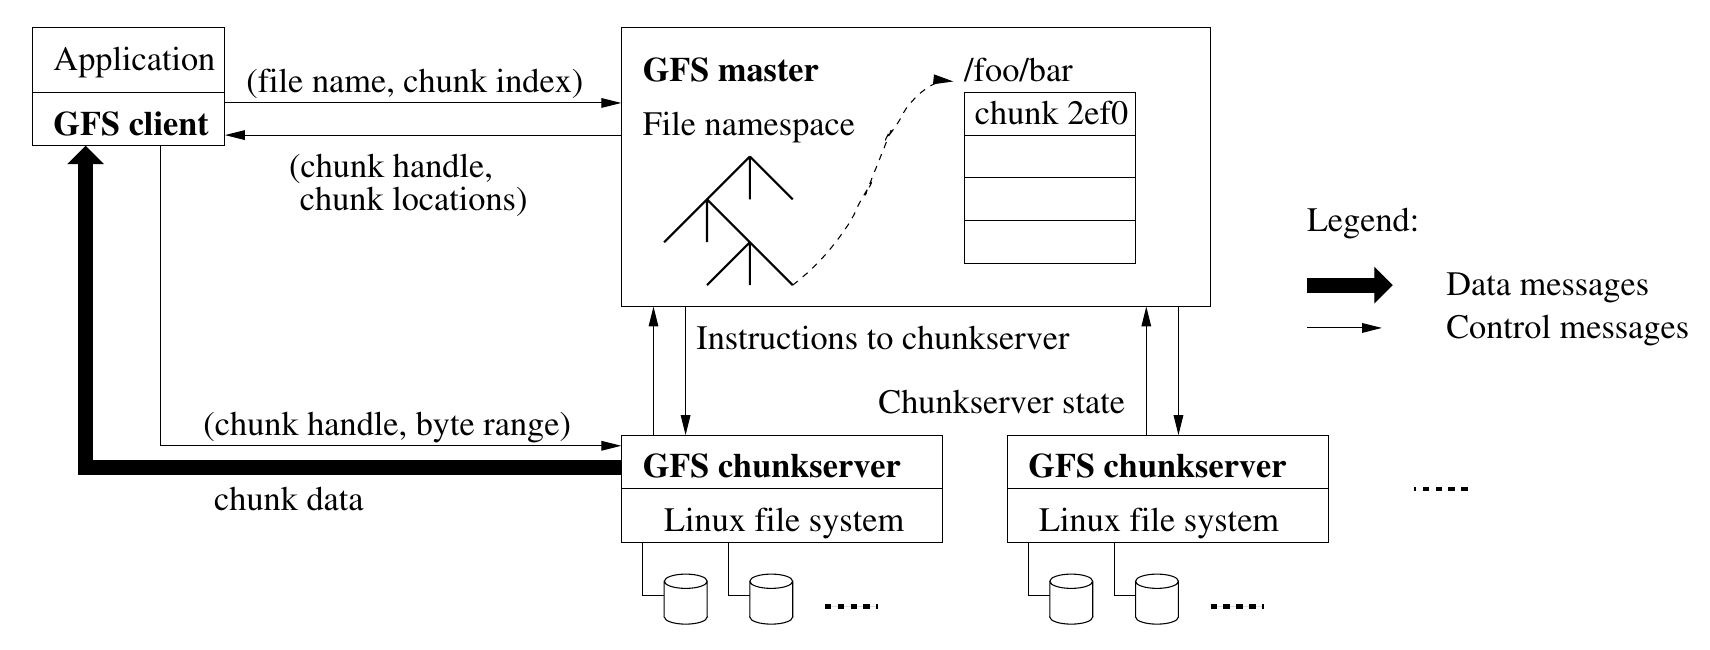
\includegraphics[width=0.96\textwidth]{figures/original/gfs-figure-1-architecture.png}
  \captionsetup{justification=centering}
  \renewcommand{\figurename}{Figure}
  \caption{GFS架构}
  \label{fig:gfs-architecture}
\end{figure*}

\subsection{架构}
如Figure 1所示，一个GFS集群由单个master和多个chunkserver组成，并由
多个客户端访问。它们通常都作为用户态进程的运行在普通的Linux服务器上。
只要机器资源允许，并且能够接受由于运行可能不太稳定的应用程序代码而带
来的可靠性下降，那么在同一台机器上同时运行chunkserver和client是很容易的。
\emph{(译者注：事实上Google的MapReduce机器会和chunkserver混合部署，
目的是尽量减少Map阶段的带宽消耗)}

文件被划分为固定大小的chunk。每个chunk都由master在创建时分配的、
不可变且全局唯一的64位chunk handle标识\emph{(译者注：它不是文件offset，
也不是文件名，也不是磁盘地址，而是master给某个chunk分配的一个64位标识符)}。chunkserver将chunk作为
Linux文件存储在本地磁盘上，并根据chunk handle和字节范围读取或写入
chunk数据。为保证可靠性，每个chunk都会复制到多个chunkserver上。
默认情况下，我们保存3个replica；不过用户可以为文件命名空间的不
同区域指定不同的复制级别。\emph{(译者认为此处指可以给不同的路径树前缀，
设置单独的replica数，比如告诉/critical/这个路径下面的所有子文件都要5 replica)}

master维护所有文件系统元数据，包括命名空间\emph{(译者认为namespace
可以理解成目录树信息)}、访问控制信息、从文件到
chunk的映射，以及chunk的当前位置。它还控制全系统范围的活动，例如
chunk lease管理、孤立chunk的垃圾回收，以及chunk在不同chunkserver之间
的迁移。master会定期通过HeartBeat消息与每个chunkserver通信，向其
发送指令并收集其状态。

每个应用程序中的GFS客户端代码实现了文件系统API，并代表应用程序
与master和chunkserver通信以读写数据。客户端在执行元数据操作时与master
交互，但所有承载数据的通信都会直接发送到chunkserver。我们不提供POSIX
API，因此无需hook到Linux vnode层。

客户端和chunkserver都不缓存文件数据。客户端缓存带来的收益很小，因为
大多数应用会流式遍历超大文件，或其工作集大到无法被缓存。不缓存文件数据
能够消除缓存一致性问题，从而简化客户端和整个系统(不过，客户端会缓存
元数据)。chunkserver也无需缓存文件数据，因为chunk以本地文件形式存储，
Linux的缓冲区缓存已经会将频繁访问的数据保留在内存中。

\subsection{单个主控(master)服务器}
单个master极大简化了我们的设计，并使master能够利用全局信息做出
复杂的chunk放置和复制决策。然而，我们必须尽量减少它参与读取和写入
的程度，以免它成为瓶颈。客户端绝不会经由master读取或写入文件数据。
相反，客户端会询问master应联系哪些chunkserver，并在有限时间内缓存
这些信息，随后直接与chunkserver交互来完成许多操作。

下面结合Figure 1说明一次简单读取的交互过程。首先，客户端根据固定的chunk
大小，将应用程序指定的文件名和字节offset转换为该文件中的chunk索引，
\\\emph{
译者注：chunk索引计算公式：
\[
\left\lfloor \frac{\text{offset}}{64 \times 1024 \times 1024} \right\rfloor
\]}
然后，它向master发送一个包含文件名和chunk索引的请求。master返回相应
的chunk handle及replica位置。客户端使用文件名和chunk索引作为键，缓存
这些信息。

接着，客户端向其中一个replica发送请求，通常会选择距离最近的replica。请求
中包含chunk handle和该chunk内的字节范围。在缓存信息过期或文件被重新
打开之前，对同一个chunk的后续读取不再需要客户端与master交互。

实际上，客户端通常会在同一个请求中查询多个chunk，而master也可以返回
紧随这些chunk之后的chunk信息。这些额外信息几乎不增加成本，却能避免
之后多次客户端与master之间的交互。

\subsection{Chunk大小}
Chunk大小是关键设计参数之一。我们选择了64MB，这远大于典型的
文件系统块大小。每个chunk replica都作为普通Linux文件存储在
chunkserver上，并且只在需要时扩展。延迟(lazy)空间分配避免了内部碎片造成的空间浪费；
而内部碎片可能正是人们反对采用如此大chunk大小的最大理由。\emph{（译者注：
这里作者是在回应大chunk可能带来的空间浪费问题。64MB是chunk的逻
辑上限和管理粒度，并不意味着每创建一个chunk replica就会立刻占用64MB磁盘
空间。由于chunk replica只是普通Linux文件，并且只会随着实际写入而扩展
，因此即使最后一个chunk没有写满，也不会必然浪费完整的64MB空间。
这里的内部碎片指的是固定大chunk可能导致的未使用空间浪费，而不是内存碎片）}

较大的chunk大小具有几个重要优点。第一，同一chunk上的读写只需
在开始时向master请求一次chunk位置信息，因此它减少了客户端与
master交互的需求。对于我们的访问负载，这种减少尤其显著，因为
应用大多顺序读写大文件。即使进行小型随机读取，客户端也能轻松
缓存一个多TB工作集中全部chunk的位置信息。第二，由于客户端更可
能在一个大chunk上执行多次操作，它可以在较
长时间内保持与chunkserver之间的持久TCP连接，从而降低网络开销
\emph{(译者注：这里的意思是，应用通常会顺序访问大文件或其中一段连续区
域。chunk越大，客户端在同一个chunk内连续读写的机会越多，因此更可能复
用同一个chunkserver连接，而不是频繁查询master、切换chunk或重新
建立TCP连接)}
。第三，它减少了存储在master上的元数据规模。这使我们能够将元数据
保存在内存中，进而带来将在section2.6.1讨论的其他优点。

另一方面，即使采用延迟空间分配，大chunk大小也有缺点。一个小文件
只包含少量chunk，可能只有一个。如果许多客户端访问同一文件，存储
这些chunk的chunkserver可能成为热点。实践中，热点并不是主要问题，
因为我们的应用大多顺序读取包含多个chunk的大文件。

然而，在GFS最初被一个批处理队列系统使用时，确实出现了热点：一个
可执行文件被作为单chunk文件写入GFS，随后在数百台机器上同时启动。
存储该可执行文件的少数chunkserver被数百个并发请求压垮。我们通过提高这
类可执行文件的复制因子\emph{(译者注：简单理解为replica数量即可)}，
并让批处理队列系统错开应用
启动时间，解决了这个问题。一种潜在的长期方案是：在这类情况下允许
客户端从其他客户端读取数据。

\subsection{元数据}
master存储三类主要元数据：文件和chunk命名空间、从文件到chunk的
映射，以及每个chunk replica的位置。所有元数据都保存在master的内存中。
前两类元数据(命名空间和文件到chunk的映射)还会通过操作日志持久化。
每次变更都会记录到存放在master本地磁盘、并复制到远程机器上的操作
日志中。使用日志使我们能够简单、可靠地更新master状态，并避免在
master崩溃时出现不一致的风险。
master不会持久化存储chunk位置信息。相反，master会在启动时，以及
每当某个chunkserver加入集群时，向各个chunkserver询问其持有的
chunk。
\\\emph{译者注：master内存结构接近这样}\\
\begin{minipage}{\columnwidth}
{\scriptsize
\begin{verbatim}
Master Memory
│
├── Namespace table
│   ├── "/"             -> 目录metadata
│   ├── "/foo"
│   ├── "/foo/bar"
│   └── "/foo/bar/a.txt"-> 文件metadata
│
├── File-to-chunk table
│   └── "/foo/bar/a.txt"
│       ├── chunk index 0 -> chunk_11
│       ├── chunk index 1 -> chunk_12
│       └── chunk index 2 -> chunk_13
│
├── Chunk metadata table
│   ├── chunk_11
│   │   ├── version number
│   │   ├── lease holder, if any
│   │   └── replica位置 -> [CS1, CS4, CS8]
│   │
│   └── chunk_12
│       ├── version number
│       ├── lease holder, if any
│       └── replica位置 -> [CS2, CS5, CS9]
│
└── Chunkserver state table
    ├── CS1 -> alive, disk usage, chunks it own
    ├── CS2 -> alive, disk usage, chunks it own
    └── CS3 -> alive, disk usage, chunks it own
\end{verbatim}
}
\end{minipage}

\subsubsection{内存数据结构}
由于元数据存储在内存中，master操作速度很快。此外，master能够
方便且高效地在后台定期扫描其全部状态。这种周期性扫描用于实现
chunk垃圾回收、在chunkserver发生故障时重新复制chunk，以及为平衡
各chunkserver之间的负载和磁盘空间使用而迁移chunk。section4.3和
section4.4会进一步讨论这些活动。

这种仅将元数据存储在内存中的方案有一个潜在顾虑：chunk数量以及
整个系统的容量，会受到master可用内存大小的限制。然而在实践中，
这并不是严重限制。对于每个64MB的chunk，master维护的元数据不足
64字节。大多数chunk都是满的，因为大多数文件包含许多chunk，只有最后一个
chunk可能未被完全填满。同样，文件命名空间数据通常每个文件也只需
不足64字节，因为它通过前缀压缩紧凑地存储文件名。\emph{(译者注：
一个1TiB文件，大约需要不到1MiB的chunk元数据；关于路径名压缩，可以考虑
trie或者压缩前缀树压缩空间，现实生活中的HDFS没有压缩，并且children是
二分查找，查找某个children的时候，复杂度O(logn))}

即使为了支持更大的文件系统，需要给master增加额外内存，这个成本也是值得的；
因为将元数据保存在内存中，可以换来系统在简单性、可靠性、性能和灵活性上的收益。

\subsubsection{chunk位置}
master不会持久化记录哪些chunkserver持有某个给定chunk的replica。
它只会在启动时轮询chunkserver来获取这些信息。之后，master能够
保持信息最新，因为它控制所有chunk放置操作，并通过定期的
HeartBeat消息监控chunkserver状态。

我们最初曾尝试在master上持久化保存chunk位置信息，但后来认为，
在启动时以及之后定期向chunkserver请求这些数据要简单得多。这样
就消除了在chunkserver加入或离开集群、改名、发生故障、重启等情况
下，让master与chunkserver保持同步的问题。在拥有数百台服务器的
集群中，这些事件发生得非常频繁。

理解这一设计决策的另一种方式是：对于自身磁盘上究竟持有哪些chunk，
chunkserver拥有最终决定权。试图在master上维护这些信息的一致视图
没有意义，因为chunkserver上的错误可能导致chunk自行消失(例如某块
磁盘损坏并被禁用)，或者操作员可能会为chunkserver改名。

\subsubsection{操作日志}
操作日志包含了关键元数据变更的历史记录。它是GFS的核心组成部分。它
不仅是元数据唯一的持久化记录，同时也充当一条逻辑时间线，用来定义并
发操作的顺序。文件和chunk，以及它们的版本号(见section4.5)，都由其
创建时对应的逻辑时间唯一且永久地标识。

由于操作日志至关重要，我们必须可靠地保存它，并且只有在元数据变更被
持久化之后，才向客户端暴露这些变更。否则，即使chunk本身仍然存在，
我们实际上也会丢失整个文件系统，或丢失最近的客户端操作。因此，
我们将日志复制到多台远程机器上\emph{(译者理解这里是为了
容灾，例如保证master机器磁盘坏了不会丢失持久化数据)}，并且只有
在相应日志记录已在本地和远程都flush到磁盘后，才响应客户端操作。
master会在刷新前将多条日志记录批量合并，从而减少flush和复制对
系统整体吞吐量的影响。\emph{(译者注：可以理解为多次write fd后
才整体做一次fsync，因为一次write一次sync太慢。客户端不能只等到
master执行了write(fd, logRecord)就收到成功响应。必须等到
包含自己那条log record的batch已经在本地和远程都flush到disk才能返回
success response)}

master通过重放操作日志来恢复文件系统状态。为了尽量缩短启动时间，
我们必须让日志保持较小。当日志增长到一定大小后，master会对自身状态
创建checkpoint。这样恢复时只需从本地磁盘加载最新checkpoint，并重放此后的少量
日志记录。

checkpoint采用紧凑的类B树形式\emph{(译者注：这里没有指针，靠文件offset
维护树结构)}，可以直接映射到内存中\emph{(译者注：例如mmap)}，
用于命名空间查找\emph{(译者注：因为这是存磁盘上的，无法插入分裂，所以只读)}，
无需额外解析。这会进一步加快恢复速度，并提高可用性。\\\emph{译者注：\\
论文提到了checkpoint是一种“读取友好型的”的可直接加载进内存的类B树文件。
它如此设计有以下好处：一是无需parse，恢复速度快；二是checkpoint
可以直接读，载入内存直接可以lookup某个目录entry；三是一个节点能存很多数据，
树的层数低，查询速度快，cache好。
}

创建checkpoint可能需要一段时间，因此master的内部状态经过专门设计，可以
在不延迟新到mutation\emph{(译者注：mutation可以理解为改变系统状态的操作。
在本段master checkpoint的语境下，它主要指改变master元数据状态的操作，
例如创建文件、删除文件、分配新chunk、修改file-to-chunk映射、
更新chunk版本号或lease状态等。普通的数据写入和追加主要由
chunkserver执行；只有当它们引发master元数据变化时，
才属于这里需要被master operation log记录并进入checkpoint的mutation)}
的情况下创建新checkpoint。master会切换到一个新的
日志文件，并由单独线程创建新checkpoint。新checkpoint包含切换前的所有mutation。
对于拥有数百万文件的集群，创建过程约需一分钟。完成后，checkpoint会同时
写入本地和远程磁盘。\emph{(译者注：这里讲了构建checkpoint实际上依赖
内存数据，但是内存数据是线上使用的，为了不hang住用户的请求，这里有数据结构上的
设计。译者认为可以采用“双map法”(类似golang sync.Map的dirty)，
构建开始的时候将当前namespace结构标记为只读称为snapshot，并且开启一个新的
namespace结构current，构建线程可以读snapshot创建checkpoint；
同时master主要业务线程可以读snapshot，读写current完成
mutation。checkpoint彻底创建完毕后合并current和snapshot；还有一种
可行的办法是开启一个背景进程，专门用来读老snapshot，应用
op log，定期制作新的snapshot，这种做法不侵入master
主进程的业务逻辑，ChatGPT告诉我这种方法类似HDFS的CheckpointNode
旁路构建)}

恢复时只需要最新的完整checkpoint及其后的日志文件。较旧的checkpoint和日志文件
可以自由删除，但我们会保留少量replica以防灾难性故障。checkpoint创建期间发生
故障不会影响正确性，因为恢复代码能够检测并跳过不完整的checkpoint。

\subsection{一致性模型}

GFS采用了一种宽松的一致性模型。该模型能够很好地支持高度分布式的
应用程序，同时仍能保持实现相对简单且高效。
下面我们将讨论GFS提供的保证，以及这些保证对应用程序意味着什么。
我们还会重点说明GFS如何维持这些保证，但将具体细节留给本文的其他
部分。

\subsubsection{GFS提供的保证}
文件命名空间mutation(例如文件创建)是原子的。它们完全由master处理：
命名空间锁保证原子性和正确性(section4.1)；master的操作日志定义了
这些操作的全局全序(section2.6.3)。

\begin{center}
  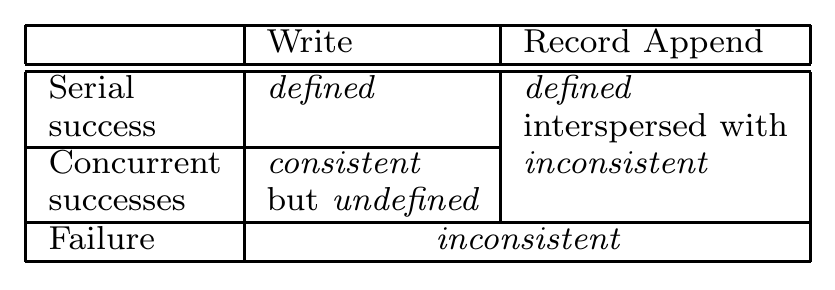
\includegraphics[width=0.95\columnwidth]{figures/original/gfs-table-1-file-region-state.png}
  \refstepcounter{table}\label{tab:file-region-state}

  {\small\textbf{Table 1.}数据mutation后的文件区域状态}
\end{center}

数据mutation\emph{(译者注：包含write和record append)}之后，
文件区域的状态取决于mutation类型、操作是成功还是
失败，以及是否存在并发mutation。Table 1总结了这些结果。如果无论客户端
从哪个replica读取，始终都能看到相同数据，则该文件区域是consistent的。
一次文件数据mutation之后，如果该区域既consistent，并且客户端能完整看到该
mutation写入的内容，则该区域是defined的。当mutation成功且未受并发写入
干扰时，受影响区域是defined的(因此也是consistent)：所有客户端始终都会看到
该mutation写入的内容。
并发成功的mutation会使该区域undefined但保持consistent：所有客户端
看到相同数据，但这些数据可能并不反映任何一个mutation实际写入的内容。
通常，它由多个mutation相互混杂的片段组成\emph{(译者注：
consistent but undefined是concurrent successes的结果，
例如client1在offset处写入AAAA，client2在offset处写入BBBB，
有可能最终的结果是AABB，最重要的原因是mutation
可能刚好跨分片，从两个客户端的角度看来，最终write函数返回的都是成功，
写出来的结果应当是AAAA or BBBB，最后读出来却可能是AABB这样的混叠数据，
这就是未定义的含义)}。
失败的mutation会使该区
域inconsistent(因此也undefined)：不同客户端可能在不同时间看到不同的数据。
下文将说明应用程序如何区分defined区域和undefined区域。应用程序无需进一步
区分undefined区域的不同种类。

数据mutation可以是\textbf{write}或\textbf{record append}。写入会
在应用程序指定的文件offset写入数据。即使存在并发mutation，\textbf
{record append}也会至少一次\emph{(译者注：这里是伏笔，以后读者会
知道如何处理重复数据保证幂等性)}原子地追加数据(即“record”)，但追加offset
由GFS选择(section3.3)，相比之下，“常规”追加只是一次写入，写入位置是客户
端认为的当前文件末尾offset，GFS会将实际offset返回给客户端；
这个offset标记了一个defined region的起始位置，而该区域包含这条记录。
此外，GFS可能会在记录之间插入padding内容\emph{(译者注：原因是
record append不能让一条record跨chunk边界；如果当前chunk剩余空间不
够放下整条record，GFS就把当前chunk剩余部分填充掉，然后让客户端到下一个
chunk重新append。实现原子append的核心设计正是“一个record不能跨chunk”，只有
一个record在一台chunk上，并且依赖chunk的pipeline串行排队执行机制
才能实现“原子append”)}，或者插入重复的record。这些padding和重复的
record占据的区域被视为inconsistent区域，并且相对于用户数据量而言通常很小。

在一系列成功的mutation之后，经过mutation的文件区域保证是defined的，
并且包含最后一次mutation写入的数据。GFS通过两种方式实现这一保证：
(a)在所有replica上以相同顺序将mutation应用到某个chunk(section3.1)；
(b)使用chunk版本号检测因chunkserver宕机期间遗漏mutation而过期的
replica(section4.5)。过期replica绝不会参与mutation，也不会被master
作为chunk位置返回给请求客户端。系统会在最早的机会对它们进行垃圾回收。

由于客户端会缓存chunk的位置信息，因此在这些缓存信息被刷新之前，
客户端可能会从一个stale replica读取数据。这个时间窗口受到两个因素限制：
一是缓存条目的超时时间，二是下一次打开该文件时会清除缓存中该文件的所有chunk信息。
此外，由于我们的多数文件都是只追加的，所以stale replica通常返
回的是一个过早的chunk结束位置\emph{(译者注：如果用户append-only而不overwrite，
当stale replica可能和primary断连后，客户端实际上最多从它这感知到early EOF，
而不是outdated data，这不是特别“危险”)}，而不是过期数据。当reader重试并联系master时，
它会立即获得当前最新的chunk位置信息。

一次成功mutation过去很久后，组件故障当然仍可能损坏或销毁数据。GFS通过
master与所有chunkserver之间的定期握手识别失效的chunkserver，并通过
校验和检测数据损坏(section5.2)。一旦问题暴露，系统会尽快从有效replica恢复数据(section4.3)。只有在GFS
来得及反应之前、通常也就是几分钟内，某个chunk的全部replica都丢失时，
该chunk才会不可逆地丢失。即使在这种情况下，它也是不可用而非被损坏：
应用程序会收到明确错误，而不是损坏的数据。

\subsubsection{对应用程序的影响}
GFS应用可以通过一些简单技术适应宽松的一致性模型。这些技术原本就因
其他目的而需要，包括依赖追加而非覆盖、创建checkpoint，以及写入可自验证、
可自标识的record。

几乎所有应用都会通过追加而非覆盖来修改文件。一种典型用法是：写入者
从头到尾\emph{(译者注：使用append)}生成一个文件，并在写完全部数据后，
原子地将文件重命名为永久名称；或者定期记录已成功写入的数据量，
形成checkpoint。checkpoint还可以包含应用层校验和。\emph{(
译者注：这里的checkpoint和之前提到的master checkpoint不是一件事，
此处指的记录某一块数据的checksum和size，告诉应用层这部分数据已经可以被
读取使用，这种边处理边读取对很多应用很有帮助)}
读取者只验证和处理截至最后一个checkpoint的文件区域，因为该区域已知处于
defined状态。即使系统存在一致性和并发的问题\emph{(译者注：这里指的是
append+checkpoint的做法)}，这套做法都很好地满足了我们的
需求。与随机写入相比，追加的效率更高，也更能抵御应用程序故障。
checkpoint使写入者可以重启后断点续写，并避免读取者处理虽然已经成功写入、但从
应用程序角度看仍不完整的文件数据。

另一种典型用法是：许多写入者并发向同一文件追加数据，以生成合并结果
或充当生产者—消费者队列\emph{(译者注：很多读者会误以为增加生产者
就能提高单个文件的append速率，实际上不是的，在同一时刻某个chunk的mutation
必须经过这个时刻“仅有一个”的primary排队，所以写入速率还是受制于primary的单机
网络、磁盘瓶颈)}。\textbf{record append}的“至少追加一次”语义能够保留每个
写入者的输出。读取者按如下方式处理偶发的padding和重复record。
写入者准备的每条record都包含校验和等额外信息，以便验证其有效性。读取者
可以使用校验和识别并丢弃额外padding和record片段。如果读取者无法容忍偶发的
重复record(例如它们会触发非幂等操作)，则可以使用record中的唯一标识符将其
过滤掉。
这些唯一标识符通常本来也需要用于命名相应的应用实体，例如Web文档。
这些record I/O相关功能(除了重复record删除之外)，都被封装在我们的
应用共享的库代码中，并且也适用于Google内部其他文件接口实现。借助这
些机制，同一串record，加上少量罕见的重复record，总是会被交付给
record reader。

\section{系统交互}
我们在设计系统时，力求将master参与所有操作的程度降至最低。在此
背景下，下面将说明客户端、master和chunkserver如何交互，以实现数据
mutation、原子\textbf{record append}和\textbf{snapshot}。

\subsection{lease与mutation顺序}
mutation是一种会改变某个chunk的内容或元数据的操作，例如普通写入或追加操作。
每个mutation都会在该chunk的所有副本上执行。我们使用lease来在各个副本之
间维持一致的mutation顺序。master会把某个chunk的lease grant给其中一个副本，
我们称这个副本为primary。primary会为该chunk上的所有mutation选择一个串行顺序。
所有副本在应用mutation时都遵循这个顺序。因此，全局mutation顺序首先由master选择的
lease顺序决定；在同一个lease内，则由primary分配的序列号决定。

lease机制旨在降低master的管理开销。lease的初始超时时间为60秒。不过，
只要chunk仍在发生mutation，primary就可以向master请求延期，并且通常
能够无限期获得延期。这些延期请求和grant lease会捎带在master与所有
chunkserver定期交换的HeartBeat消息中。master有时会尝试在lease
到期前撤销它(例如，master希望禁止对一个正在重命名的文件进行mutation时)。
即使master失去了与某个primary的通信，它也可以在旧lease到期后，
安全地向其他replica grant lease。\emph{(译者注：这里的rename更准确地说
是master对namespace映射的一次原子修改，
即把某个文件对象从旧路径绑定到新路径，而不是复制或重建文件数据。
由于GFS client可能缓存了chunk的primary/replica信息，并在已有lease
有效期内绕过master继续向primary发起append/write，master如果希望
rename成为一个清晰的发布/提交边界，就需要暂时禁止该文件上的mutation。
因此它可能在lease到期前主动revoke lease，使基于旧缓存状态的写入失效，
后续写入必须重新联系master，并基于新的namespace状态重新获得授权。你看
假如你已经rename成功了，但是去append原来的那个文件路径才是ok，岂不奇怪？)}

Figure 2通过以下带编号的步骤，展示了一次写入操作的控制流。

1. 客户端询问master：哪个chunkserver持有该chunk当前的lease，以及
   其他replica的位置。如果没有任何replica持有lease，master会向
   它选择的一个replica grant lease(此步骤未在图中展示)。

2. master返回primary的身份以及其他secondary replica的位置。客户端会
   缓存这些数据以供之后的mutation使用。只有当primary不可达，或回复
   表示自己不再持有lease时，客户端才需要再次联系master。

3. 客户端将数据推送到所有replica。推送顺序可以任意。每个chunkserver
   都会将数据保存在内部LRU缓冲区缓存中，直到数据被使用或因老化而
   被逐出。通过将数据流与控制流解耦，我们可以不受哪个chunkserver
   是primary的影响，依据网络拓扑调度开销较大的数据流，从而提升性能。
   section3.2会进一步讨论这一点。

4. 所有replica确认收到数据后，客户端向primary发送写请求。该请求标识
   先前已推送到全部replica的数据。primary为它收到的所有mutation分配
   连续序列号\emph{(译者注：master元数据的mutation顺序号/
   operation log顺序和每个chunk内data mutation的顺序是两套不同的顺序体系，
   不能混为一个全局序列)}，这些mutation可能来自多个客户端，从而提供所需的串行化。
   它按照序列号顺序将mutation应用到自己的本地状态。

5. primary将写请求转发给所有secondary replica。每个secondary replica都按照
   primary分配的相同序列号顺序应用mutation。

6. 所有secondary都会回复primary，表明自己已完成该操作。

7. primary回复客户端。任一replica遇到的错误都会报告给客户端。发生错误时，
   写入可能已经在primary和任意一个secondary replica子集上成功。(如果它
   在primary处失败，就不会获得序列号，也不会被转发。)
   客户端请求会被视为失败，修改后的区域则处于不一致状态。我们的客户端
   代码会通过重试失败的mutation来处理这类错误。它会先对步骤3到步骤7进行
   若干次尝试；若仍失败，便从写入操作的开始处重新重试。
   \\\begingroup\itshape 译者注：可以考虑一种网络隔离场景来理解该机制。
   \\假设chunk有A、B、C三个replica，当前版本号为7，A持有lease并作为primary。
   此时A与master、B、C发生网络隔离，但client仍能连接到A。client可能仍基于旧
   缓存认为A是primary，并向A发起mutation。A即使能在本地为该mutation
   排序并尝试执行，也无法把该mutation转发给B、C并获得它们的确认，因此该请
   求会被报告为失败；如果mutation只在部分replica上执行成功，则被修改
   区域处于inconsistent状态，client需要重试。

   随着A与master失联，master在旧lease过期后，可以从仍然可达且
   up-to-date的replica中选择新的primary，例如B，并推进chunk version number，
   例如从7增加到8。B、C收到新版本后继续参与后续mutation；
   A因为错过了版本更新和后续mutation，恢复后会被master识别为
   stale replica，不会再被返回给client，
   也不会参与新的mutation，之后会被垃圾回收。

   这里的关键不是多数派提交，而是：同一个chunk的mutation必须由当前有效
   lease holder排序，并由所有参与的replica按相同顺序执行；旧primary的
   lease到期后不能继续合法提交mutation，版本号则用于识别那些错过mutation
   的stale replica。
   
   这里还有一个特别关键的点，version更准确地说是chunk的一个epoch标签。
   master会用version判断哪些replica属于当前有效的副本。一次mutation需要由
   当前lease holder排序，并由master当前认可的up-to-date replicas按相同顺序执行。
   如果某个replica在version推进期间不可用，它恢复后因版本落后而被识别为stale，
   不再参与后续mutation。简单理解，version隐式蕴藏了一个“有效replica”列表，
   一次成功的mutation必须让这列表里的所有人都执行mutation。
   \endgroup

如果应用程序的写入很大，或跨越了chunk边界，GFS客户端代码会将其拆分为
多个写入操作。它们都会遵循上述控制流，但可能与其他客户端的并发操作
交错，并被其覆盖。
因此，这个共享的文件区域最终可能包含来自不同客户端的片段。不过，各replica仍然
相同，因为每个单独操作都以相同顺序在所有replica上成功完成。正如
section2.7所述，这会使文件区域处于consistent但undefined的状态。

\begin{figure}[t]
  \centering
  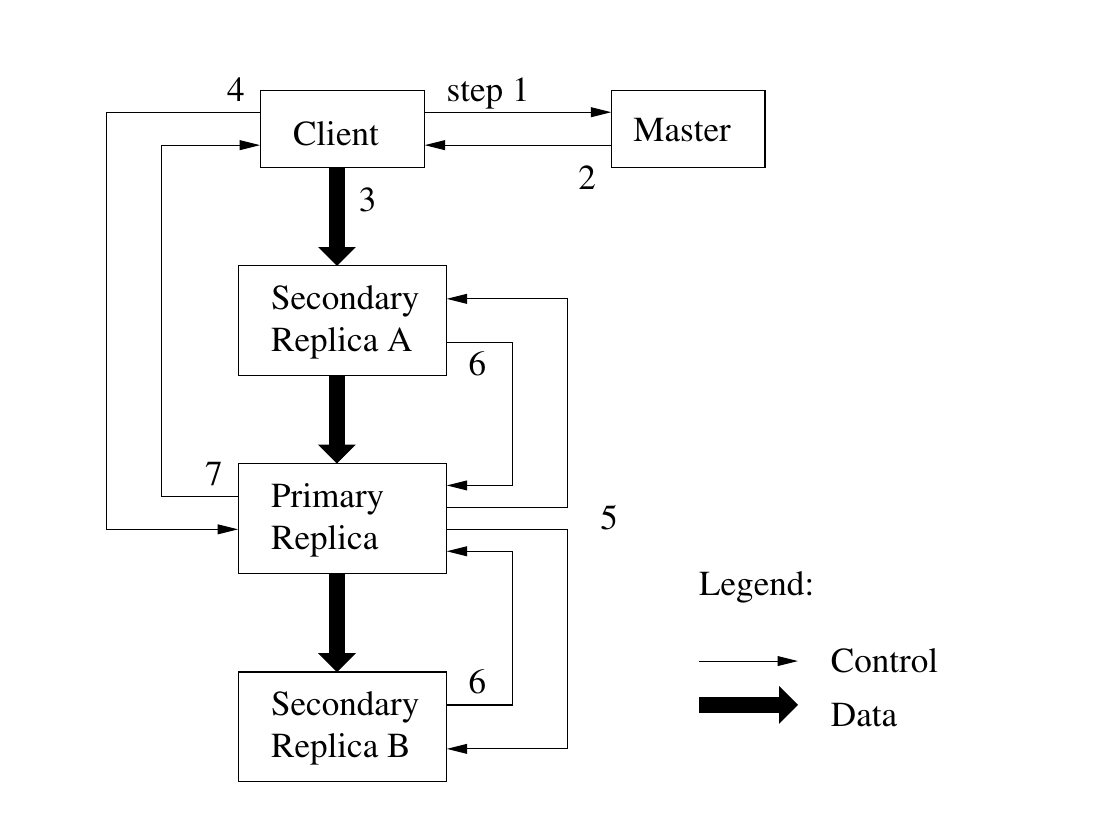
\includegraphics[width=0.95\columnwidth]{figures/original/gfs-figure-2-write-control-data-flow.png}
  \captionsetup{justification=centering}
  \renewcommand{\figurename}{Figure}
  \caption{写入控制流和数据流}
  \label{fig:gfs-write-control-data-flow}
\end{figure}

\subsection{数据流}
我们将数据流与控制流解耦，以高效利用网络。控制流从客户端流向
primary，再流向所有secondary；而数据则以流水线方式，沿着精心选择的
chunkserver链线性推送。我们的目标是充分利用每台机器的网络带宽，避免
网络瓶颈和高延迟链路，并尽量缩短推送全部数据所需的延迟。

为了充分利用每台机器的网络带宽，数据会沿着一条chunkserver链线性
推送\emph{(译者注：例如Client->A->B->C)}，而不是以其他拓扑结
构(例如树形结构)分发。这样，每台机器的全部
出站带宽都会用于尽快传输数据，而不是把出口带宽分摊给多个接收者\emph{(
译者注：一台机器的出口宽带是有限的。实际上别的场景上，Fan-Out在架构上一般
不是什么好设计，译者在实际的工程中，例如IM群聊场景也有这样的体会，
Fan-Out架构会让群聊发送接口成为瓶颈——大量的CPU损耗和网络开销)}。

为了尽可能避开网络瓶颈和高延迟链路(例如交换机之间的链路通常同时具备
这两个问题)，每台机器都会将数据转发给网络拓扑中距离最近、且尚未收到
数据的机器。假设客户端正在向chunkserver S1到S4推送数据，它会先将
数据发送给最近的chunkserver，例如S1。
S1会将数据转发给S2到S4中距离自己最近的chunkserver，例如S2。类似地，
S2会将数据转发给S3或S4中距离S2更近的一个，如此继续。我们的网络拓扑
足够简单，因此可以根据IP地址准确估计这些“距离”。

最后，我们通过在TCP连接上对数据传输进行流水线化来降低延迟。一旦
chunkserver收到一部分数据，就会立即开始转发。流水线对我们特别有用，
因为我们使用具有全双工链路的交换网络。立即发送数据不会降低接收速率。
在没有网络拥塞时，向R个replica传输B字节数据的理想耗时为B/T+RL，其中T
是网络吞吐量，L是字节在两台机器间传输的延迟。我们的网络链路通常为
100Mbps(T)，而L远小于1ms。因此，理想情况下，分发1MB数据大约需要
80ms。

\subsection{原子\textbf{record append}}
GFS提供了一种称为\textbf{record append}的原子追加操作。在传统写入中，
客户端指定数据要写入的offset。对同一区域的并发写入无法串行化：该区域
最终可能包含来自多个客户端的数据片段。
而在\textbf{record append}中，客户端只指定数据。GFS会在它选择的offset处，
\textbf{至少一次}原子地将数据追加到文件中(即作为一段连续字节序列)，
并将该offset返回给客户端。这类似于在Unix中向以O\_APPEND模式打开的文件写入
数据，即使是多个writer并发写入，也不会出现竞争而产生的“交叉文本”。
\\\emph{(译者注：这里作者实际是在说Unix O\_APPEND文件写入和GFS
的record append语义相似，都是原子追加。然而，其实GFS的语义又
和Unix O\_APPEND不完全一样。第一点是GFS的record append保证的是
\textbf{至少一次}，也就是两个线程并发追加内容，一个写hello，一个写world，
那么真实在GFS里面的内容可能是hellohelloworld，或者helloworldhelloworld。
你看，它虽然保证了一个record原子被插入，但是是多少次呢？答案是GFS只保证一次。而且
最需要注意的是，插入后也许在chunk server不同的机器上读，会读出不同的结果。
这里埋下伏笔，我将在后续提到这个badcase。这个“乱序问题”很微妙，但是也可以被解决)}

\textbf{record append}被我们的分布式应用大量使用：不同机器上的许多客户端会并发向同一
文件追加数据。如果使用传统写入，它们就需要额外进行复杂且昂贵的同步，
例如通过分布式锁管理器完成同步。在我们的工作负载中，这类文件通常充当
多生产者/单消费者队列，或保存来自许多不同客户端的合并结果。
\\\begingroup\itshape
译者注：

例如chunk10是文件的最后一个chunk，primary是server A。
客户端尝试向该chunk执行record append时，如果A发现该chunk的剩余空间
不足以容纳完整record，GFS不会把这条record拆开跨chunk存放，而是由A
将chunk10的剩余部分填充为padding，并通知其他副本执行同样的padding mutation。
随后客户端需要在下一个chunk上重试record append——也就是客户端需要请求master，
找master创建下一个chunk的元信息。

这里体现了GFS record append的一个设计取舍：为了保证一条record作为连续字节序列
原子地落在某个chunk内，GFS接受了chunk边界处可能产生padding和重试的代价。
由于GFS写入流程是先push data到各副本，再请求primary执行mutation，
当大量客户端并发append且当前chunk接近满时，可能会出现一批已经push到旧chunk
但最终无法写入的无效数据传输。

不过，这不意味着GFS不支持多生产者追加。相反，GFS的record append正是为了支持
多个客户端并发向同一文件追加记录。但单个文件的当前active chunk只有一个primary
负责排序和分配offset，因此单文件写入吞吐不能随着writer数量线性扩展。若需要更高
写入吞吐，通常应采用分片输出或多个队列文件，而不是让所有producer写入同一个文件。
\endgroup

\textbf{record append}是一种mutation，它遵循section3.1中的控制流，只是在primary处
增加了一些额外逻辑。客户端将数据推送到文件最后一个chunk的所有replica，
然后向primary发送请求。primary会检查：在当前chunk执行\textbf{record append}是否会使
其超过最大大小(64MB)。
如果会超过，primary会将chunk填充到最大大小，通知secondary执行相同操作，
并回复客户端，表示应在下一个chunk上重试该操作。(\textbf{record append}被限制为至多
最大chunk大小的四分之一，以将最坏情况下的碎片控制在可接受范围内)。
如果\textbf{record}能够容纳在最大大小内(这是通常情况)，primary会将数据追加到自己
的replica中，通知secondary在与primary完全相同的offset写入数据，最后向
客户端回复成功。

如果\textbf{record append}在任一replica上失败，客户端会重试该操作。因此，同一chunk的
replica可能包含不同数据，也可能全部或部分包含同一\textbf{record}的重复内容。GFS并不
保证所有replica在字节层面完全相同；它只保证数据至少会作为一个原子单元被
写入一次。
这一性质直接来自一个简单事实：要让操作报告成功，数据必须已在某个chunk
的所有replica上的相同offset处被写入。并且在此之后，所有replica的长度至少会
达到\textbf{record}结尾。因此，即使之后由不同replica成为primary，任何未来\textbf{record}都会
被分配到更高的offset，或被分配到不同chunk。
按照我们的一致性保证，成功的\textbf{record append}操作写入数据的区域是已定义的
(因此也是一致的)，而其间的区域则是inconsistent的(因此也是未定义的)。正如
section2.7.2所讨论的，我们的应用可以处理inconsistent区域。
\\\emph{译者注：回收之前的伏笔。读者可以去看Youtube观看Raft2020 Lec3 GFS视频，
在1h10分处它讲解了一个由于失败重试，导致的“乱序问题”，它是一个很神奇的badcase。
\\在真实的应用中，我们会使用append record
来做追加的数据写入，读取则是从头读到已consistent的区域，然后从头到尾扫描“自标识”特征来识别record
——这样可以剔除无用padding或者record之间的garbage信息。但是这里教授的例子
很微妙，它描述了一种非常奇妙的现象：多个writer append record同一个GFS File时，假如一次写入尝试因为
“只有部分replica成功append”而失败，后续客户端重试，会留下“脏数据”，而这个脏数据也是合理的自标识数据。
因此，就算业务层自己做了record自标识识别，也做了去重，但是在不同的机器可能会消费到不同的record顺序。
所以怎么解决呢？一是可以干脆就不让多人写一个GFS文件了，事实上HDFS就是这么做的，它将lease做到了客户端和
master上，保证同时只有一个客户端向一个文件append；二是可以改造GFS，我可以提供一些想法：可以尝试
让所有机器都成为primary的复制状态机，每当primary上任的时候，强制让其它secondary同步自己经历过的mutation，
不允许出现分岔。读者可以多思考思考复制状态机以及Raft的No-op Entry优化，从这两个角度入手改造GFS。}

\subsection{\textbf{snapshot}}
\textbf{snapshot}操作几乎可以瞬时创建一个文件或目录树(即“source”)的replica，同时尽量
减少对正在进行的mutation的干扰。用户使用它快速创建超大数据集的分支
replica(并且经常递归地创建这些replica的replica)，或在试验某些之后可轻松提交
或回滚的修改前，对当前状态创建检查点。

与AFS[5]类似，我们使用标准的\textbf{copy-on-write}技术实现\textbf{snapshot}。当master收到\textbf{snapshot}
请求时，首先会撤销即将创建\textbf{snapshot}的文件中所有chunk尚未到期的lease。这样
可以确保之后对这些chunk的任何写入，都必须与master交互以找到lease持有者。
这使master有机会先创建该chunk的新replica。

待lease被撤销或到期后，master会将该操作记录到磁盘。然后，它通过复制
source文件或source目录树的元数据，将这条日志记录应用到内存状态中。新创建的
\textbf{snapshot}文件与source文件指向相同的chunk。

在\textbf{snapshot}操作之后，客户端首次想要写入chunk C时，会向master请求当前lease
持有者\emph{(译者注：举个好例子，假如正在append，客户端对primary有所缓存，但是在此
刻chunk lease被收回，客户端写入时会发现not primary，此时会去请求master寻找新的primary)}。
master发现chunk C的引用计数大于1。它会暂缓回复客户端请求，
转而选择一个新的chunk handle C'。随后，它要求每个持有C当前replica的
chunkserver创建一个名为C'的新chunk\emph{(译者注：lease是master调用chunkserver
实现的，笔者认为创建C'时可以夹带copy-on-write信息，通知它进行复制)}。
通过在与原chunk相同的chunkserver上创建新chunk，我们确保数据可以在
本地复制，而无需经由网络传输(我们的磁盘速度大约是100Mb以太网链路的
3倍)。从此以后，请求处理与任何普通chunk都没有区别：master将新chunk C'的lease grant给
其中一个replica，然后回复客户端。客户端随后可以像平常一样写入该chunk，
而不会察觉它刚刚是从一个现有chunk创建出来的。
\\\emph{译者注：snapshot在用户视角那里其实就是像拷贝了一个文件夹，但是这个拷贝
特别快，该文件夹下面的所有文件的所有chunk lease都会被revoke掉。读者可能会担心
这里会有惊群效应客户端来拿lease会引发惊群效应。可以这样考虑：
1.读客户端不需要lease，只有正在写的客户端需要来重新拿；2.用户可以选择只snapshot
一个小文件夹，尽量避免snapshot整个目录树，避免惊群。}

\section{master服务器操作}
master执行所有命名空间操作。此外，它还管理整个系统中的chunk replica：
负责做出放置决策、创建新的chunk及其replica，并协调各种全系统范围的
活动，以保持chunk具有完整replica、平衡所有chunkserver之间的负载，并回收
未使用的存储空间。下面将分别讨论这些主题。

\subsection{命名空间管理与锁}
许多master操作可能耗时很长。例如，\textbf{snapshot}操作必须撤销\textbf{snapshot}所覆盖的全部
chunk上的chunkserver lease。我们不希望这些操作运行时阻塞其他master
操作。因此，我们允许多个操作同时处于活动状态，并使用命名空间区域上的
锁来确保正确的串行化。

与许多传统文件系统不同，GFS没有一种列出目录中全部文件的、按目录划分的
数据结构\emph{(译者注：读者参考“元数据”一节的设计，它更像是维护的一个
fullpath->metadata信息的映射，并没有按目录划分的树结构)}。
它也不支持同一个文件或目录的别名(即Unix术语中的硬链接或
符号链接)。在逻辑上，GFS将命名空间表示为一张从完整路径名映射到元数据
的查找表。通过前缀压缩，这张表可以高效地存储在内存中。命名空间树中的每个节点(绝对文件名或绝对目录名)
都关联着一个读写锁。

每个master操作在运行前都会获取一组锁。通常，若操作涉及
\textbf{/d1/d2/.../dn/leaf}，它会对目录名\textbf{/d1}、\textbf{/d1/d2}、...、
\textbf{/d1/d2/.../dn}获取读锁，并对完整路径名\textbf{/d1/d2/.../dn/leaf}
获取读锁或写锁。请注意，\textbf{leaf}可以是文件，也可以是目录，具体取决于操作类型。

下面说明
这一加锁机制如何防止在将\textbf{/home/user}创建\textbf{snapshot}到\textbf{/save/user}期间，
创建文件\textbf{/home/user/foo}。
\textbf{snapshot}操作会对\textbf{/home}和\textbf{/save}获取读锁，并对\textbf{/home/user}和
\textbf{/save/user}获取写锁。文件创建操作会对\textbf{/home}和\textbf{/home/user}
获取读锁，并对\textbf{/home/user/foo}获取写锁。由于两个操作都会尝试获取
\textbf{/home/user}上相互冲突的锁，它们会被正确地串行化。
文件创建无需在父目录上获取写锁，因为不存在需要防止修改的“目录”或
类似inode的数据结构。名称上的读锁已足以防止父目录被删除。

该加锁方案的一个优点是：它允许在同一目录中并发进行mutation。例如，
可以在同一目录中并发创建多个文件：每个操作都会获取目录名上的读锁，
以及文件名上的写锁。目录名上的读锁足以防止该目录被删除、重命名或创建
\textbf{snapshot}。文件名上的写锁会将两次尝试创建同名文件的操作串行化。

由于命名空间可能
拥有许多节点，读写锁对象会按需延迟分配，并在不再使用时删除。此外，为了
防止死锁，锁会按一致的全序获取：先按命名空间树中的层级排序，同一层级内
再按字典序排序。

\subsection{replica放置}
一个GFS集群在多个层面上都具有高度分布性。它通常拥有分布在许多机器
机架上的数百个chunkserver。这些chunkserver又可能被来自同一机架或不同
机架的数百个客户端访问。位于不同机架的两台机器之间通信时，可能需要
跨越一个或多个网络交换机。
此外，一个机架的进出带宽可能低于该机架内所有机器总带宽的总和。
多层级的分布式结构给数据分布带来了独特挑战：既要保证可扩展性，又要保证可靠性和可用性。

chunk replica放置策略有两个目的：最大化数据可靠性和可用性，以及最大化网络
带宽利用率。对于这两个目标，仅将replica分散到不同机器上并不够。这样做只能
防范磁盘或机器故障，并充分利用每台机器的网络带宽。
我们还必须将chunk replica分散到不同机架上。这确保即使整个机架受损或离线，
某个chunk的部分replica仍能存活且可用。例如，机架可能因网络交换机或供电
线路等共享资源故障而离线。
这种做法还意味着，某个chunk的流量，尤其是读取流量，可以利用多个机架的
聚合带宽\emph{(译者注：前面提到了机架的带宽是较小的，因此从多个机架下载
会有更大的带宽，读者别忘了secondary机器同样可以下chunk)}。
另一方面，写入流量必须跨越多个机架传输；这是我们愿意接受的权衡。

\subsection{创建、重新复制与负载均衡}
创建chunk replica有三个原因：创建chunk、重新复制和重新均衡。

master创建chunk时，需要选择最初为空的replica应放置在哪里。它会考虑多个
因素。(1)我们希望将新replica放在磁盘空间利用率低于平均水平的
chunkserver上。长期来看，这会使各chunkserver之间的磁盘利用率趋于
均衡。
(2)我们希望限制每个chunkserver上“最近”创建的数量。虽然创建本身
开销很小，但它能可靠地预示即将到来的大量写入流量：chunk是在写入需要时
创建的；而在我们“追加一次、读取多次”的访问负载中，chunk一旦被完全
写入，通常就几乎成为只读的。
(3)如前所述，我们希望将一个chunk的replica分散到不同机架上。

一旦可用replica数量低于用户指定的目标值，master就会重新复制该chunk。
出现这种情况可能有多种原因：某个chunkserver变得不可用
\emph{(译者注：比如“lease与mutation顺序”提到的primary挂掉的场景，若心跳检测
超时，master会认为它上面的chunk不再availabel。后续如果需要一个新lease会
重新选出一个primary并且赋予lease，version随即+1，此时其实该chunk就只有两个可用replica了。
同理，如果secondary挂掉，此时master感知到了，也会标记为unavailbel，
当需要lease的时候也会进行grant new lease，通知其它chunk server：
“目前只剩下这两个replica了”。读者可以清晰地察觉到这里其实有一个lazy grant lease
的设计，即使是chunk机挂了，也不必马上重建lease，等需要的时候重建也很ok)}；
它报告自己的replica可能已损坏；其一块磁盘因错误被禁用；或者复制目标值被提高。
每个需要重新复制的chunk都会根据多个因素确定优先级。其中之一是它距离
复制目标值的差距。例如，丢失两个replica的chunk会比只丢失一个replica的chunk
获得更高优先级。此外，相比属于最近删除文件的chunk，我们优先重新复制
仍然存活的文件的chunk(section4.4)(\emph{译者注：读者可能会好奇为什么已经删除的文件
也有复制优先级，难道它也要复制？是的，因为GFS的删除其实是给一个“Deleted At”的标记然后改个名字，
到时间了再删除，这样即使文件被错误地删除了也能抢救回来})。
最后，为了尽量减少故障对正在运行的应用程序的影响，任何阻塞客户端进展
的chunk都会被提高优先级。

master选择优先级最高的chunk，并通过指示某个chunkserver直接从现有有效
replica复制chunk数据，来“克隆”它。新replica的放置目标与创建时类似：均衡
磁盘空间利用率、限制单个chunkserver上的同时进行的克隆操作，并将replica分散到
不同机架。
为了防止克隆流量挤占客户端流量，master会限制整个集群以及每个
chunkserver上的同时进行的克隆操作数量。此外，每个chunkserver都会通过限制
向源chunkserver发出的读取请求数量，来限制其为每次克隆操作使用的带宽。

最后，master会定期重新对副本负载均衡：它检查当前replica分布，并迁移replica以获得
更好的磁盘空间和负载均衡。通过这一过程，master还能逐步填充新的
chunkserver，而不是向新机器立即塞满大量新chunk及以及随之而来的大量写入流量。
新replica的放置条件与前文所述类似。此外，master还必须选择要删除的现有
replica。通常，它倾向于删除位于可用空间低于平均水平的chunkserver上的
replica，以均衡磁盘空间使用率。
\\\emph{译者注：这里很好懂，意思是一个新上任的chunkserver磁盘使用量很低
按照优先级算法，replica会成为“hotspot”，所以需要master进行渐进的、逐步的
负载均衡。}

\subsection{垃圾回收}
文件被删除后，GFS不会立即回收其占用的物理存储空间。它只会在文件和
chunk两个层级的定期垃圾回收过程中，以延迟方式回收这些空间。
我们发现，这种做法使系统更加简单，也更加可靠。

\subsubsection{机制}
当应用程序删除文件时，master会像处理其他变更一样，立即记录删除操作。
但是，它不会立即回收资源，而是仅将文件重命名为包含删除时间戳的隐藏
名称。在master定期扫描文件系统命名空间时，如果这类隐藏文件已存在超过
3天，就会将其移除(该时间间隔可配置)。在此之前，文件仍可通过新的特殊名
称读取，也可以通过将其重命名回普通名称来恢复删除。当隐藏文件
从命名空间中移除时，其内存元数据也会被清除。这实际上切断了它与
全部chunk之间的链接。

在对chunk命名空间进行类似的定期扫描时，master会识别孤立chunk(即无法
从任何文件到达的chunk)，并删除这些chunk的元数据。每个chunkserver会在
与master定期交换的HeartBeat消息中，报告自己持有的一部分chunk。
master会回复所有已不再存在于自身元数据中的chunk标识。chunkserver可以
自由删除这类chunk的replica。

\subsubsection{讨论}
在编程语言的语境中，分布式垃圾回收是一个需要复杂解决方案的难题；但在
我们的场景中，它相当简单。我们可以轻松识别全部指向chunk的引用：它们
位于完全由master维护的文件到chunk映射中。我们也能轻松识别全部chunk replica：
它们是每个chunkserver指定目录下的Linux文件。
任何master未知的这类replica都是“垃圾”。

与急切删除相比，采用垃圾回收方式回收存储空间有几个优点。第一，在组件
故障频繁的大规模分布式系统中，它简单且可靠。chunk创建可能只在部分
chunkserver上成功，从而留下master不知道存在的replica。replica删除消息
可能丢失，而master必须记得在自身或chunkserver发生故障后
重新发送这些消息。垃圾回收提供了一种统一且可靠的方式，用于清理所有
已知无用的replica。第二，它将存储回收合并到master的常规后台活动中，例如定期扫描命名空间
以及与chunkserver握手。因此，回收以批处理方式完成，成本可以被分摊。
此外，只有在master相对空闲时才执行回收，使master能够更及时地响应
需要快速处理的客户端请求。第三，延迟回收存储空间可以为意外且不可逆的删除提供一层安全保护。


根据我们的经验，主要缺点是：当存储空间紧张时，这种延迟有时会妨碍用户
精细调整存储使用。反复创建和删除临时文件的应用，可能无法立即复用已
释放的存储空间。我们通过以下方式处理这些问题：如果一个已删除文件被显式再次删除，就
加速其存储回收。我们还允许用户对命名空间的不同部分应用不同的复制和
回收策略。例如，用户可以指定某个目录树内文件的全部chunk不进行复制，并且任何被
删除的文件都立即且不可逆地从文件系统状态中移除。
\\\emph{译者注：
\\GFS的文件删除实际上就是打了一个“Deleted At”的标，并且重命名，等到三天后它才不
可逆地被master“遗忘”。在master遗忘后，就通过心跳“懒加载”地告诉chunk servers某个
文件已经删除了，chunk此时才能被chunk server从磁盘中删除。这里说的是可以选择给不同
目录设置不同的回收策略，比如某个critial文件夹5天回收；
而temp文件夹立马回收。
\\此外这里还提到了之前就已经说过的可按目录配置副本数的功能，可以给/tmp设置较少的副本数
(甚至是1)，来让它少复制甚至不复制，这样可以缓解磁盘资源紧张的问题。
}

\subsection{过期replica检测}
如果某个chunkserver发生故障，并在宕机期间遗漏了对某个chunk的
mutation，那么该chunk的replica可能变得过期(stale)。对于每个chunk，master都会
维护一个chunk版本号，用于区分最新replica和过期replica。

每当master为某个chunk grant新的lease时，都会提高该chunk的版本号，并
通知最新replica。master和这些replica都会将新版本号记录到各自的持久化状态中。
这一过程发生在通知任何客户端之前，因此也发生在客户端能够开始向该chunk
写入之前。
如果另一个replica当前不可用，它的chunk版本号就不会被推进。当该
chunkserver重启并报告其持有的chunk集合及对应版本号时，master会发现
它持有过期replica。如果master看到的版本号高于自身记录的版本号，master会
假定自己在grant lease时曾发生故障，并将较高版本视为最新版本。
\emph{
\\译者注：\\
这里特别微妙，grant lease过程中，master先在内存中生成new\_version=current\_version+1，
随即master将该“换届”信息告知给primary和secondary，这些replicas都会持久化version。
接下来master就把这个chunk version的推进持久化写入op log。请注意上述过程的任
何部位都可能宕机，因此要精细地考虑到所有边界情况。
\\在master重启后，它做的事情是：
\\1.从checkpoint+op log恢复metadata，包括namespace目录树，file->chunks mapping
以及chunk handle到chunk的mapping信息(这里信息也包括chunk version)。
\\2.从所有chunkserver上报中汇聚信息，包括chunk version和locations，补充自己的
内存结构。若遇到比自己持久化的version小的，直接视为stale；若遇到比自己version大的
直接采用；但是如果发现全部都比自己小的话，只能告诉用户这个chunk不可用了。
\\3.进入正轨，处理请求，补副本，进行垃圾回收。
\\此外，读者可以注意，此处master假如发现机器宕机，不论是primary还是secondary，都不会
立刻进行新的grant lease，它只会默默地标记这个机器unavailabel了。等下一次进行写入操作需要
lease的时候，才会进行新的grant lease——这完完全全又是一个“懒加载”的思想，避免一台机器挂掉
需要处理大量的grant lease，而导致master“惊群”。
}

master会在定期垃圾回收中删除过期replica。在此之前，当它回复客户端的
chunk信息请求时，实际上会将过期replica视为完全不存在。
作为另一层保护，master会在通知客户端哪个chunkserver持有某个chunk的
lease时，附带该chunk的版本号；或者，在克隆操作中指示某个chunkserver
从另一个chunkserver读取该chunk时，也会附带版本号。
客户端或chunkserver执行操作时会验证版本号，从而确保其访问的始终是
最新数据。
\section{容错与诊断}
在设计该系统时，我们面临的最大挑战之一，是处理频繁发生的组件故障。
组件的质量和数量共同决定了：这些问题是常态而非例外。我们既不能完全
信任机器，也不能完全信任磁盘。
组件故障可能导致系统不可用，或者更糟的是导致数据损坏。下面将讨论我们
如何应对这些挑战，以及当问题不可避免地发生时，系统内置了哪些用于诊断
问题的工具。

\subsection{高可用性}
在GFS集群的数百台服务器中，任意时刻都必然有部分服务器不可用。我们
通过两种简单但有效的策略保持整个系统的高可用性：快速恢复和复制。

\subsubsection{快恢复}
无论是master还是chunkserver，都被设计为无论以何种方式终止，都能在数秒
内恢复状态并启动。事实上，我们不区分正常终止和异常终止；服务器通常只需
直接杀死进程即可关闭。
客户端和其他服务器只会经历一次轻微停顿：它们等待尚未完成的请求超时，
重新连接到已重启的服务器，然后重试。section6.2.2报告了实际观察到的
启动时间。

\subsubsection{chunk复制}
如前所述，每个chunk都会复制到位于不同机架的多个chunkserver上。用户
可以为文件命名空间的不同部分指定不同的复制级别，默认值为3。
当chunkserver离线，或通过校验和验证检测到replica损坏时(见section5.2)，
master会按需克隆现有replica，以确保每个chunk始终具有完整replica。
尽管复制一直很好地满足了我们的需求，但随着只读存储需求不断增长，我们
正在探索其他跨服务器冗余形式，例如奇偶校验或纠删码。
由于我们的流量主要由追加和读取构成，而不是小型随机写入，我们预计在
这个非常松耦合的系统中实现这些更复杂的冗余方案虽有挑战，但仍然可控。

\subsubsection{master复制}
master状态通过复制来保证可靠性。它的操作日志和检查点会复制到多台机器
上。只有当状态mutation对应的日志记录已在本地和所有master replica上刷新到
磁盘后，该mutation才被视为已提交。
为简单起见，一个master进程始终负责全部mutation，以及垃圾回收等会在
系统内部改变状态的后台活动。当它发生故障时，可以几乎立即重启。如果它
所在的机器或磁盘发生故障，GFS外部的监控基础设施会在其他位置利用已复制
的操作日志启动一个新的master进程。
客户端只使用master的规范名称(例如gfs-test)。该名称是一个DNS别名；
如果master被迁移到另一台机器，该别名可以被修改。

此外，即使primary master宕机，“shadow”master仍可向文件系统提供只读
访问。它们是shadow而非mirror，因为它们可能略微落后于primary，通常只
落后几分之一秒。
对于未被积极mutation的文件，或不介意得到略旧结果的应用程序，shadow
master能够提高读取可用性。事实上，由于文件内容是从chunkserver读取的，
应用程序不会观察到过期的文件内容。
在短暂窗口中可能过期的是文件元数据，例如目录内容或访问控制信息。

为了保持信息更新，shadow master会读取持续增长的操作日志replica，并像
primary一样，将完全相同的变更序列应用到自己的数据结构中。与primary
相同，它会在启动时(以及此后不频繁地)轮询chunkserver以定位chunk replica，
并与它们频繁交换握手消息来监控状态。
shadow master只依赖primary master提供replica位置更新；这些更新源于
primary关于创建和删除replica的决策。

\subsection{数据完整性}
每个chunkserver都使用校验和来检测已存储数据的损坏。考虑到一个GFS集群
通常在数百台机器上拥有数千块磁盘，它会经常遇到磁盘故障；这些故障会在
读取和写入路径上造成数据损坏或丢失。(其中一个原因见section7。)
我们可以使用其他chunk replica从损坏中恢复，但通过比较不同chunkserver上的
replica来检测损坏并不现实。此外，replica之间存在差异也可能是合法的：GFS的
mutation语义，特别是前文讨论的原子\textbf{record append}，并不保证replica
完全相同。因此，每个chunkserver都必须通过维护校验和，独立验证自身replica
的完整性。

一个chunk被划分为64KB的块，每个块都有对应的32位校验和。和其他元数据
一样，校验和保存在内存中，并通过日志持久化存储；它们与用户数据分开保存。

对于读取操作，chunkserver会在向请求方返回任何数据前，验证与读取范围
重叠的数据块的校验和。无论请求方是客户端还是另一个chunkserver，都遵循
这一规则。因此，chunkserver不会将损坏传播到其他机器。
如果某个块与记录的校验和不匹配，chunkserver会向请求方返回错误，并向
master报告该不匹配。随后，请求方会从其他replica读取，master则会从另一个
replica克隆该chunk。新的有效replica就位后，master会指示报告不匹配的
chunkserver删除自己的replica。

出于几个原因，校验和对读取性能影响很小。由于大多数读取至少跨越数个块，
为了验证，我们只需额外读取并计算校验和的相对少量数据。GFS客户端代码还
会尽量将读取对齐到校验和块边界，以进一步降低这部分开销。
此外，chunkserver上的校验和查找与比较不需要任何I/O，而校验和计算通常
能够与I/O操作重叠执行。

对于追加到chunk末尾的写入(而非覆盖已有数据的写入)，校验和计算得到了
高度优化，因为它们在我们的工作负载中占主导地位。我们只需增量更新最后
一个未填满的校验和块的校验和，并为追加操作填满的任何全新校验和块计算
新的校验和。
即使最后一个未填满的校验和块已经损坏，而我们此时未能检测到，新校验和
值也不会与已存储数据匹配；下次读取该块时，仍会像往常一样检测到损坏。

相反，如果写入覆盖了chunk中的一个现有范围，我们必须先读取并验证被
覆盖范围的第一个和最后一个块，再执行写入，最后计算并记录新的校验和。
如果在部分覆盖首尾块前不验证它们，新校验和可能会掩盖未被覆盖区域中
原本存在的损坏。

在空闲期间，chunkserver可以扫描并验证不活跃chunk的内容。这使我们能够
检测很少被读取的chunk中的损坏。一旦检测到损坏，master就可以创建一个
新的未损坏replica，并删除损坏replica。
这样可以避免一个不活跃但已损坏的chunk replica误导master，使其以为某个
chunk已经拥有足够数量的有效replica。

\subsection{诊断工具}

广泛且细致的诊断日志，对问题隔离、调试和性能分析带来了极大帮助，
而成本却很低。没有日志，很难理解机器之间短暂且无法复现的交互。
GFS服务器会生成诊断日志，记录许多重要事件(例如chunkserver上线和
下线)，以及全部RPC请求和回复。删除这些诊断日志不会影响系统正确性。
不过，只要存储空间允许，我们会尽量保留这些日志。

RPC日志包含网络上传输的精确请求与响应，但不包含正在读取或写入的文件
数据。通过匹配请求和回复，并整理不同机器上的RPC记录，我们可以重建
完整的交互历史，从而诊断问题。
这些日志也可作为负载测试和性能分析的追踪记录。

日志记录对性能的影响很小(且远小于它带来的收益)，因为这些日志以顺序、
异步方式写入。最近发生的事件还会保存在内存中，可供持续在线监控。
\section{性能评测}
本节将给出若干微基准测试，用以说明GFS架构和实现中固有的瓶颈；
同时也会展示Google正在使用的真实集群的一些数据。

\subsection{微基准测试}
我们在一个由1个master、2个master replica、16个chunkserver和16个客户端组成的GFS
集群上测量性能。请注意，这一配置是为便于测试而搭建的。典型集群拥有数百个chunkserver和数百个客户端。

所有机器均配置双1.4GHz的PIII处理器、2GB内存、两块80GB、5400转/分的磁盘，以及一条连
接到HP2524交换机的100Mbps全双工以太网链路。19台GFS服务器机器全部连接到一台交换机，
16台客户端机器全部连接到另一台交换机。这两台交换机之间通过一条1Gbps链路相连。

\subsubsection{读}
N个客户端同时从文件系统读取数据。每个客户端从一个320GB的文件集合中随机读取一个4MB区域。
该操作重复256次，因此每个客户端最终读取1GB数据。
全部chunkserver的内存总量只有32GB，因此我们预计Linux缓冲区缓存的命中率最多为10\%。
我们的结果应当接近冷缓存条件下的结果。

Figure 3(a)展示了N个客户端的聚合读取速率及其理论上限。该上限取决于
先达到饱和的资源：当两台交换机之间的1Gbps链路饱和时，聚合速率上限为125MB/s；
当单个客户端的100Mbps网络接口饱和时，每个客户端的上限为12.5MB/s。
只有一个客户端读取时，观测到的读取速率为10MB/s，即单客户端上限的80\%。
当有16个读取者时，聚合读取速率达到94MB/s，约为125MB/s链路上限的75\%，即每个客户端约6MB/s。
效率从80\%下降到75\%，是因为随着读取者数量增加，多个读取者同时从同一个chunkserver
读取数据的概率也会增加。

\subsubsection{写}
N个客户端同时向N个不同文件写入数据。每个客户端通过一系列1MB
写入，向一个新文件写入1GB数据。Figure 3(b)展示了聚合写入速率
及其理论上限。该上限稳定在67MB/s，因为每个字节都需要写入16个
chunkserver中的3个，而每个chunkserver的入站连接速率为12.5MB/s。

单个客户端的写入速率为6.3MB/s，约为该上限的一半。造成这一结果的主要原因是我们的网络栈。
它与我们用于向chunk replica推送数据的流水线方案配合得不够好。从一个replica向另一个replica传播数
据时产生的延迟，降低了整体写入速率。

当有16个客户端时，聚合写入速率达到35MB/s(即每个客户端2.2MB/s)，约为理论上限的一半。
与读取情况相同，随着客户端数量增加，多个客户端并发写入同一个chunkserver的可能性也会提高。
此外，16个写入者发生冲突的可能性高于16个读取者，因为每次写入涉及3个不同replica。

写入速度低于我们的预期。在实践中，这并未成为主要问题：尽管它会增加单个客户端所感知的延迟，
但并不会显著影响系统向大量客户端提供的聚合写入带宽。

\subsubsection{Record Append}
Figure 3(c)展示了\textbf{record append}的性能。N个客户端同时向同一个文件追加数据。
性能受存储该文件最后一个chunk的chunkserver网络带宽限制，与客户端数量无关。
单个客户端时速率为6.0MB/s；当客户端数增加到16个时，速率降至4.8MB/s，主要原因是网络拥塞，
以及不同客户端观察到的网络传输速率波动。

我们的应用通常会并发生成多个这样的文件。换言之，N个客户端会同时向M个共享文
件追加数据，其中N和M都达到数十或数百的规模。因此，实验中出现的chunkserver
网络拥塞在实践中并不是显著问题，因为当某个文件对应的chunkserver忙碌时，客户端仍
可以继续写入另一个文件。

\subsection{真实世界的集群}
我们现在考察Google内部正在使用的两个集群，它们可代表其他若干类似集群。
集群A由一百多名工程师定期用于研究与开发。一个典型任务由人工用户发起，
运行时间最长可达数小时。它读取数MB到数TB的数据，对数据进行转换或分析，
并将结果写回集群。集群B主要用于生产数据处理。任务持续时间更长，并且只需偶尔
人工干预，就能持续生成和处理数TB规模的数据集。在两种情况下，一个“任务”都
由分布在多台机器上的许多进程构成，它们会同时读写大量文件。

\subsubsection{存储}
如Table 2的前五项所示，两个集群都拥有数百台chunkserver，提供数十TB的磁盘空间，
且磁盘使用率较高但尚未完全占满。“已用空间”包含所有chunk replica。几乎所有文件都保存了3个
replica。因此，这两个集群分别存储了18TB和52TB的文件数据。

两个集群的文件数量相近，不过集群B中已删除文件所占比例更高，即已被删除或被新
版本替换、但其存储空间尚未回收的文件。由于其中的文件往往更大，它也拥有更多chunk。

\begin{center}
  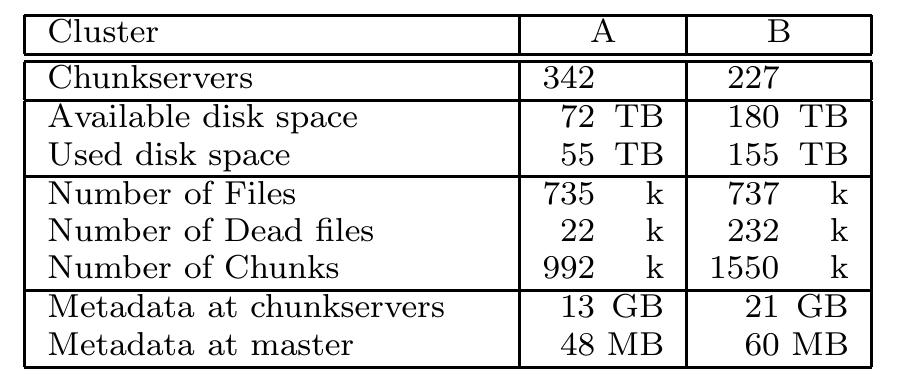
\includegraphics[width=0.95\columnwidth]{figures/original/gfs-table-2-cluster-characteristics.png}
  \refstepcounter{table}\label{tab:gfs-cluster-characteristics}

  {\small\textbf{Table 2.}两个GFS集群的特征}
\end{center}

\subsubsection{元数据}
所有chunkserver合计存储数十GB的元数据，其中大部分是用户数据64KB块的校验和。
chunkserver保存的另一类元数据只有section4.5讨论过的chunk版本号。

master保存的元数据要小得多，只有数十MB，平均每个文件约100字节。这与我们的假设一致：
在实践中，master的内存大小不会限制系统容量。每个文件的大部分元数据是以前缀压缩形式
保存的文件名。其他元数据包括文件所有权和权限、文件到chunk的映射，以及每个chunk的当前版本。
此外，对于每个chunk，我们还保存当前replica位置和用于实现写时复制的引用计数。

每台服务器，无论是chunkserver还是master，都只保存50MB到100MB的元数据。
因此恢复速度很快：服务器只需从磁盘读取这些元数据数秒，便能够响应查询。
不过，master在从所有chunkserver获取chunk位置信息之前，仍会在一段时间内受到限制，
通常为30到60秒。

\begin{figure*}[t]
  \centering
  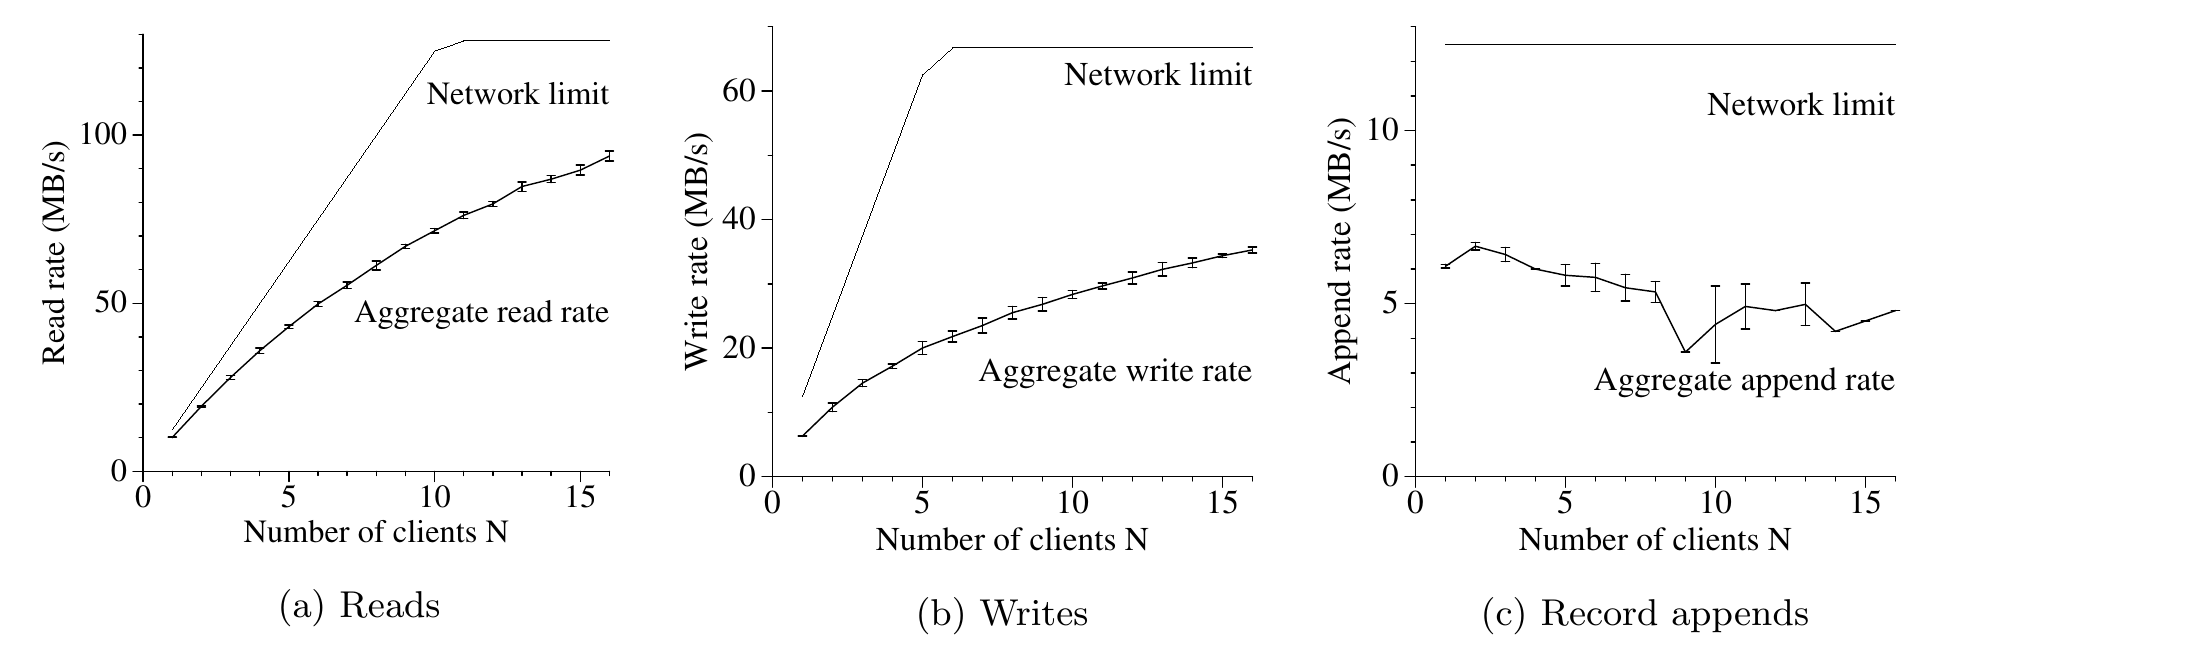
\includegraphics[width=0.96\textwidth]{figures/original/gfs-figure-3-aggregate-throughputs.png}
  \captionsetup{justification=centering}
  \renewcommand{\figurename}{Figure}
  \caption{聚合吞吐量。上方曲线表示网络拓扑带来的理论上限；下方曲线表示测得的吞吐量。误差线表示95\%置信区间；由于测量方差较低，部分误差线难以辨认。}
  \label{fig:gfs-aggregate-throughputs}
\end{figure*}

\subsubsection{读写速率}
Table 3展示了不同时间段内的读写速率。进行这些测量时，两个集群均已运行约一周。
(这些集群不久前曾为升级到新版GFS而重启)

自重启以来，平均写入速率低于30MB/s。我们进行这些测量时，集群B正处于一段写入活动
突发期，产生约100MB/s的数据；由于写入会传播到3个replica，这导致了300MB/s的网络负载。

\begin{center}
  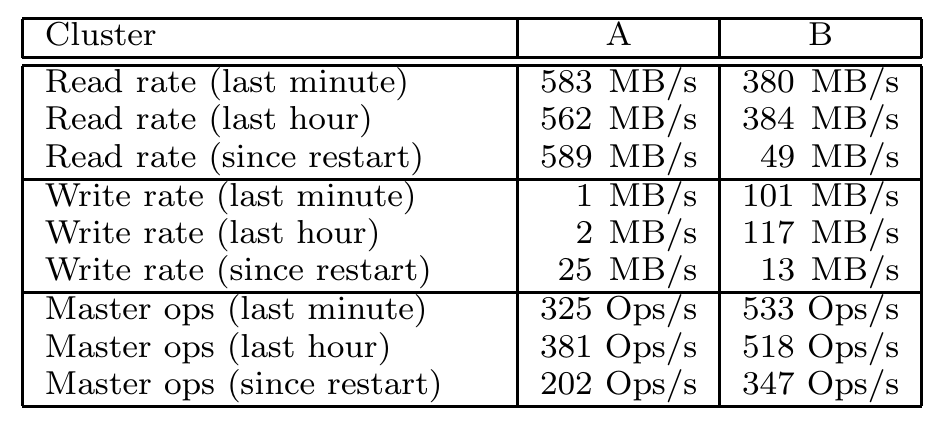
\includegraphics[width=0.95\columnwidth]{figures/original/gfs-table-3-performance-metrics.png}
  \refstepcounter{table}\label{tab:gfs-performance-metrics}

  {\small\textbf{Table 3.}两个GFS集群的性能指标}
\end{center}

读取速率远高于写入速率。正如我们所假设的，整体访问负载中读取操作多于写入操作。
两个集群当时都处于高强度读取活动期间。特别是，集群A在此前一周一直维持580MB/s的读取速率。
它的网络配置可支持750MB/s，因此资源利用较为高效。集群B可支持1300MB/s的峰值读取速率，
但其应用实际只使用了380MB/s。

\subsubsection{master负载}
Table 3还表明，发送给master的操作速率约为每秒200到500次。master可以轻松处理这一速率，
因此不会成为这些访问负载的瓶颈。

在较早版本的GFS中，master偶尔会成为某些访问负载的瓶颈。它大部分时间都在顺序扫
描大型目录(其中包含数十万个文件)，以查找特定文件。此后，我们修改了master的数据结
构，使其能够在命名空间中进行高效的二分查找。现在，它可以轻松支持每秒数千次文件访
问。如有必要，我们还可以在命名空间数据结构之前设置名称查找缓存，进一步提高速度。

\subsubsection{恢复时间}
在一个chunkserver发生故障后，部分chunk会变为replica不足，必须通过克隆恢复其replica数量。
恢复所有这类chunk所需的时间取决于可用资源数量。在一项实验中，我们终止了集群B中
的一台chunkserver。该chunkserver保存约15,000个chunk，共含600GB数据。为限制对运
行中应用的影响，并为调度决策预留余量，我们的默认参数将该集群限制为最多同时执行91个克隆操
作(chunkserver数量的40\%)，且每个克隆操作最多可使用6.25MB/s(50Mbps)的带宽。
所有chunk在23.2分钟内恢复完成，有效复制速率为440MB/s。

在另一项实验中，我们终止了两台chunkserver，每台大约保存16,000个chunk和660GB数据。
这次双重故障使266个chunk只剩下一个replica。我们以更高优先级克隆这266个chunk，
并在2分钟内全部将其恢复到至少2倍replica，使集群能够在不丢失数据的情况下承受另一台
chunkserver故障。


\subsection{访问负载拆解}
本节将详细拆解两个GFS集群上的访问负载。这两个集群与section6.2中的集群具有可比性，
但并不完全相同。集群X用于研究与开发，集群Y用于生产数据处理。

\subsubsection{方法与注意事项}

这些结果只包含由客户端发起的请求，以便反映我们的应用为整个文件系统产生的访问负载。
它们不包括为执行客户端请求而产生的服务器间请求，也不包括内部后台活动，例如转发
写入或负载再平衡。

I/O操作的统计数据基于从GFS服务器记录的实际RPC请求中，以启发式方法重建的信息。
例如，GFS客户端代码可能会将一次读取拆分为多个RPC，以提高并行度；我们据此推断出
原始读取。由于我们的访问模式高度程式化，我们预计任何误差都会落入噪声范围。由应
用显式记录日志或许能提供稍微更准确的数据，但从实际操作角度看，重新编译并重启数千
个正在运行的客户端并不可行，而且从如此多机器收集结果也十分繁琐。

不应过度泛化我们的访问负载。由于Google同时完全控制GFS及其应用，应用往往会针对GFS进
行调优；反过来，GFS也是为这些应用设计的。这种相互影响也可能存在于通用应用之间。

\begin{center}
  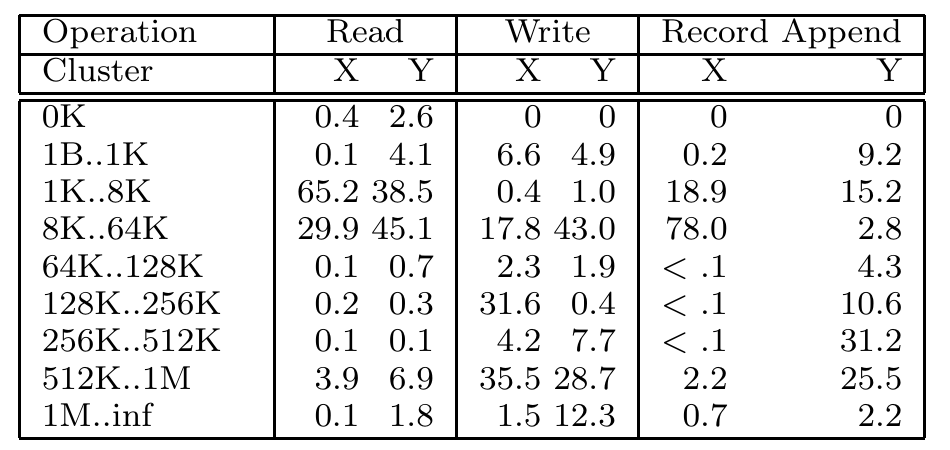
\includegraphics[width=0.95\columnwidth]{figures/original/gfs-table-4-operations-by-size.png}
  \refstepcounter{table}\label{tab:gfs-operations-by-size}

  {\small\textbf{Table 4.}按操作大小划分的操作占比(\%)}
\end{center}

\subsubsection{chunkserver访问负载}
Table4展示了按大小划分的操作分布。读取大小呈现双峰分布。
小读取(小于64KB)来自寻道密集型客户端，它们会在巨大文件中查找小片数据。
大读取(大于512KB)则来自对整个文件进行的长时间顺序读取。

集群Y中有相当数量的读取完全不返回数据。我们的应用，特别是生产系统中的应用，
常将文件用作生产者-消费者队列。生产者并发向文件追加数据，而消费者读取文件末尾。
当消费者的速度超过生产者时，偶尔会没有数据返回。集群X较少出现这种情况，因为它
通常用于短生命周期的数据分析任务，而非长生命周期的分布式应用。

写入大小同样呈现双峰分布。大写入(大于256KB)通常源于写入端进行了较大规模的缓冲。
缓冲数据较少、更频繁地进行checkpoint或同步、或者生成数据较少的写入端，会产生较小的写
入(小于64KB)。

对于\textbf{record append}，集群Y中大型\textbf{record append}所占比例远
高于集群X，因为使用集群Y的生产系统针对GFS进行了更积极的调优。

Table5展示了不同大小操作传输的数据总量。对于所有类型的操作，较大的操
作(大于256KB)通常占据大部分传输字节。由于随机寻道访问负载，小读取(小于64KB)也会
传输一部分虽小但不可忽略的读取数据。

\begin{center}
  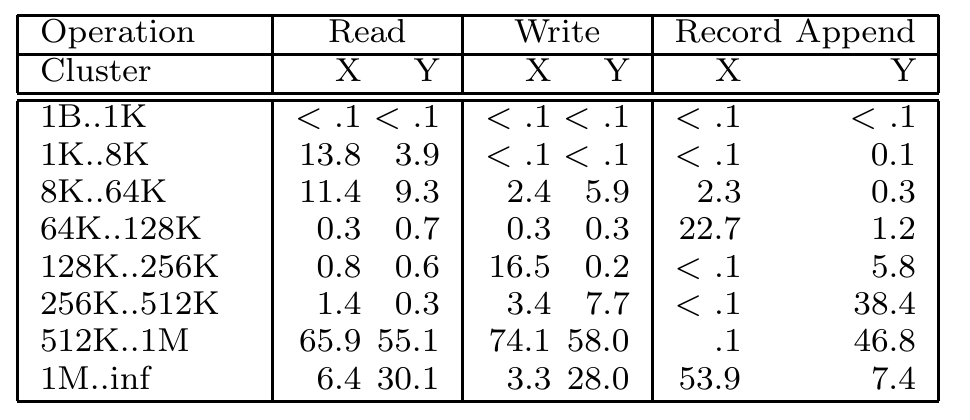
\includegraphics[width=0.95\columnwidth]{figures/original/gfs-table-5-bytes-transferred-by-operation-size.png}
  \refstepcounter{table}\label{tab:gfs-bytes-transferred-by-operation-size}

  {\small\textbf{Table 5.}按操作大小划分的传输字节数占比(\%)。对于读取操作，大小指
  实际读取并传输的数据量，而非请求的数据量。如果读取操作尝试读取超过文件末尾的数据，
  这两者可能不同；按照设计，这种情况在我们的访问负载中并不少见。}
\end{center}

\begin{center}
  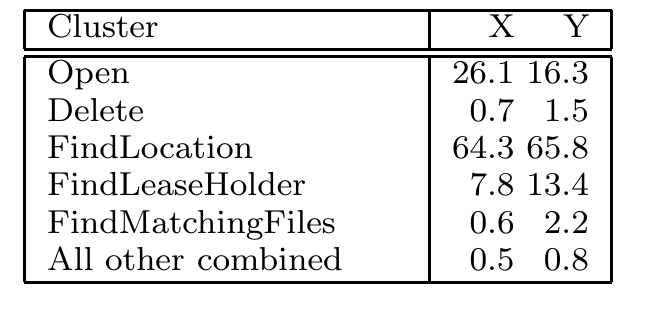
\includegraphics[width=0.82\columnwidth]{figures/original/gfs-table-6-master-requests-by-type.png}
  \refstepcounter{table}\label{tab:gfs-master-requests-by-type}

  {\small\textbf{Table 6.}按类型划分的master请求占比(\%)}
\end{center}

\subsubsection{append vs write}
\textbf{record append}被广泛使用，尤其是在我们的生产系统中。对于集群X，按传输字节
数计算，写入与\textbf{record append}的比例为10:1；按操作次数计算，比例为8:1。
对于用于生产系统的集群Y，这两个比例分别为3.7:1和2.5:1。此外，这些比例表明，两个集群
中的\textbf{record append}通常都比\textbf{write}更大。然而，对于集群X，在测量期间
\textbf{record append}的总体使用量相当低，因此结果很可能被一两个采用特
定缓冲区大小选择的应用所扭曲。

正如预期，我们的数据mutation访问负载以追加而非覆盖为主。我们测量了
primary replica上被覆盖的数据量。这近似于客户端有意覆盖此前写入的数据，而非追
加新数据的情形。对于集群X，覆盖操作占mutation字节数的不足0.0001\%，占
mutation操作数的不足0.0003\%。对于集群Y，这两个比例均为0.05\%。尽管
这一比例极小，但仍高于我们的预期。结果发现，大部分覆盖来自客户端因错误或超时而进行
的重试。它们本身并不属于访问负载，而是重试机制带来的结果。

\subsubsection{master访问负载}
Table 6展示了发送给master的请求按类型划分的构成。大多数请求用于读取时获取
chunk位置(\textbf{FindLocation})，以及进行数据mutation时获取lease持有者信
息(\textbf{FindLeaseLocker})。

集群X与Y的\textbf{Delete}请求数量显著不同，这是因为集群Y存储的生产数据集会定期重
新生成并由新版本替换。其中一部分差异还隐藏在\textbf{Open}请求数量的差异中，
因为文件的旧版本可能会在从头以写入模式打开时被隐式删除(按Unix的\textbf{open}术语，即\textbf{"w"}模式)。

\textbf{FindMatchingFiles}是一种支持\textbf{ls}及类似文件系统操作的模式匹配请求。
与其他发往master的请求不同，它可能需要处理命名空间中的很大一部分，因此开销可能较高。
集群Y更频繁地出现此类请求，因为自动化数据处理任务往往需要检查文件系统的某些部分，
以了解全局应用状态。相比之下，集群X中的应用受用户更明确的控制，通常会预先知道所有
所需文件的名称。

\section{经验}

在构建和部署GFS的过程中，我们遇到过各种问题，其中一些属于运维问题，另一些属于技术问题。

起初，GFS被设想为生产系统的后端文件系统。随着时间推移，其使用范围扩展到研究与开发任务。
它最初几乎不支持权限、配额等功能，但现在已经具备这些功能的初步形式。生产系统通常纪律
严明、管理受控，但用户有时并非如此。我们需要更多基础设施来防止用户彼此干扰。

我们遇到的一些最大问题与磁盘和Linux有关。许多磁盘向Linux驱动程序声明支持一系列
IDE协议版本，但实际上只有在较新的版本下才能可靠响应。由于这些协议版本非常相似，
这些硬盘大多数时候可以正常工作；但偶尔，版本不匹配会导致硬盘与内核对硬盘状态产生分歧。
内核中的问题会因此悄无声息地损坏数据。这个问题促使我们使用校验和来检测数据损坏；
与此同时，我们修改了内核，以处理这些协议不匹配的情况。

此前，由于\textbf{fsync()}的开销，我们在Linux2.2内核上遇到过一些问题。其开销与文
件大小成正比，而不是与被修改部分的大小成正比。对于我们的大型操作日志而言，这
尤其是在实现checkpoint之前是一个问题。我们一度通过使用同步写入来规避它，最终迁
移到了Linux2.4。

另一个Linux问题是单个读写锁：地址空间中的任何线程从磁盘换入页面时需要持有它(读锁)，
或者在\textbf{mmap()}调用中修改地址空间时需要持有它(写锁)。我们曾在轻负载下观察到系统出
现瞬态超时，并仔细排查资源瓶颈或偶发的硬件故障。最终，我们发现，当磁盘线程正在换
入先前已映射的数据时，这把单独的锁会阻塞主网络线程将新数据映射到内存中。由于我们
的主要限制来自网络接口，而非内存拷贝带宽，我们以额外一次拷贝为代价，
将\textbf{mmap()}替换为\textbf{pread()}，从而规避了这个问题。

尽管偶尔会遇到问题，Linux代码的可用性仍多次帮助我们探索并理解系统行为。在适当情
况下，我们会改进内核，并将这些改动分享给开源社区。

\section{相关工作}

与其他大型分布式文件系统(例如AFS[5])一样，GFS提供位置无关的命名空间，
使数据能够为了负载均衡或容错而被透明地迁移。与AFS不同，为了提供聚合性能并提升容错能力，
GFS以更接近xFS[1]和Swift[3]的方式，将一个文件的数据分布到多个存储服务器上。

由于磁盘相对廉价，并且复制比更复杂的RAID[9]方案更简单，GFS目前只使用复制来提供冗余。
因此，它比xFS或Swift消耗更多原始存储空间。

与AFS、xFS、Frangipani[12]和Intermezzo[6]等系统不同，GFS不在文件系统接
口之下提供任何缓存。我们的目标工作负载在单次应用运行中几乎没有数据复用，
因为它们要么流式处理大型数据集，要么在其中随机寻道，并且每次只读取少量数据。

一些分布式文件系统，例如Frangipani、xFS、明尼苏达大学的GFS[11]和GPFS[10]，
移除了中心化服务器，并依赖分布式算法实现一致性与管理。我们选择中心化方案，以简化设计、
提高可靠性并获得灵活性。特别是，中心化master使实现复杂的chunk放置与复制策略容易得多，
因为master已经拥有大部分相关信息，并控制这些信息如何变化。我们通过保持master状态较小，
并将其完整复制到其他机器上来实现容错。目前，可扩展性与读取高可用性由我们的
shadow master机制提供。对master状态的更新通过追加到预写日志而持久化。因此，
我们可以采用类似Harp[7]的primary-copy方案，提供比当前方案具有更强一致性保证的高可用性。

在向大量客户端提供聚合性能方面，我们处理的问题与Lustre[8]类似。
不过，我们专注于应用需求，而非构建符合POSIX的文件系统，因此显著简化了这个问题。
此外，GFS假设系统由大量不可靠组件构成，因此容错是设计的核心。

GFS与NASD架构[4]最为相似。NASD架构以网络附加磁盘驱动器为基础，而GFS如NASD
原型一样，使用普通机器作为chunkserver。与NASD工作不同，我们的chunkserver
使用延迟分配的固定大小chunk，而非可变长度对象。此外，GFS实现了负载再平衡、
复制与恢复等生产环境所需的功能。

与明尼苏达大学的GFS和NASD不同，我们并不试图改变存储设备模型。
我们关注利用现有普通组件，满足复杂分布式系统日常的数据处理需求。

原子\textbf{record append}支持的生产者-消费者队列，
解决了与River[2]中分布式队列类似的问题。River使用分布在多台机器上的内存队列
和精细的数据流控制，而GFS使用可由多个生产者并发追加的持久化文件。
River模型支持m对n的分布式队列，但缺少持久化存储带来的容错能力；
GFS则只能高效支持m对1的队列。多个消费者可以读取同一文件，但必须协调对输入负载的划分。

\section{结论}

Google File System展现了在普通硬件上支撑大规模数据处理工作负载所必需的特性。
尽管某些设计决策是针对我们独特环境作出的，但其中许多决策也适用于规模和成本敏感
度相近的数据处理任务。


我们从当前及预期的应用工作负载和技术环境出发，重新审视了传统文件系统的假设。
这些观察使我们在设计空间中选择了截然不同的方案。我们将组件故障视为常态而非例外，
针对主要以追加方式写入(可能是并发追加)、随后读取(通常为顺序读取)的巨大文件进行优化，
并通过扩展和放宽标准文件系统接口来改进整个系统。

我们的系统通过持续监控、复制关键数据以及快速自动恢复来提供容错能力。
chunk复制使我们能够容忍chunkserver故障。这些故障的频率促使我们设计了一种新的
在线修复机制，它会定期且透明地修复损坏，并尽快补偿丢失的replica。此外，我们使用校验
和检测磁盘或IDE子系统层面的数据损坏；考虑到系统中的磁盘数量，这类问题已经变得十分常见。

我们的设计能够向执行各种任务的大量并发读取者和写入者提供高聚合吞吐量。
我们通过将经由master的文件系统控制，与直接在chunkserver和客户端之间进行
的数据传输分离，实现这一目标。大chunk大小和chunk lease减少了master对常见
操作的参与；其中chunk lease将数据mutation中的权限委托给primary replica。
这使得我们能够采用简单的中心化master，同时避免其成为瓶颈。我们相信，对网络栈的
改进将消除当前单个客户端写入吞吐量的限制。

GFS已成功满足我们的存储需求，并在Google内部广泛用作研究与开发以及生产数据处理的
存储平台。它是一项重要工具，使我们能够持续创新，并解决整个Web规模的问题。

\section*{致谢}
\noindent
我们感谢以下人员对系统或论文作出的贡献。Brian Bershad(我们的论文指导人)
以及匿名评审者提出了宝贵意见和建议。Anurag Acharya、Jeff Dean和David desJardins
参与了早期设计。Fay Chang完成了跨chunkserver replica比较相关的工作。
Guy Edjlali负责存储配额。Markus Gutschke完成了测试框架和安全性增强相关工作。
David Kramer负责性能改进。Fay Chang、Urs Hoelzle、Max Ibel、
Sharon Perl、Rob Pike和Debby Wallach对论文早期草稿提出了意见。
Google的许多同事勇敢地将数据托付给这个新文件系统，并提供了有用反馈。Yoshka参与了早期测试。


\nocite{*}
\bibliographystyle{unsrt}
\bibliography{references}
\end{document}
